% Copyright (c) 2005-2008 Center for Urban Simulation and Policy Analysis,
% University of Washington.  Permission is granted to copy, distribute and/or
% modify this document under the terms of the GNU Free Documentation License,
% Version 1.2 or any later version published by the Free Software Foundation;
% with no Invariant Sections, no Front-Cover Texts, and no Back-Cover Texts.
% A copy of the license is included in the section entitled "GNU Free
% Documentation License".

% This is the root latex source file for the Opus and UrbanSim Users Guide.
% The guide is organized as a set of 'include' files, normally one file
% per chapter.  It uses the Python latex documentation standards and latex
% definition files -- see http://www.python.org/doc/current/doc/doc.html
% Also see the "Writing Documentation" chapter in this manual for more
% information.


\part{Modeling components}\label{part-user-guide}

\chapter{Data in Opus}
\label{chap:data-in-opus}

\emph{This chapter is under construction...}

Datasets are analogous to tables in a database. Attributes
are analogous to columns in a database table. e.g. geographical
datasets, households...

\section{Primary and Computed Attributes}

\section{Importing and Exporting Data}

\chapter{Creating Variables in Opus}


Opus is implemented in the Python programming language, so we begin
with a review of the language in Section \ref{sec:python}. Numpy is a numerical library for Python that is used exensively in the
Opus system, so this is covered in Section \ref{sec:numpy}. Using
Python and Numpy, many of the Opus Variables are coded as modules, and
these are explained in Section \ref{sec:variables}.  Finally, a recent
and extremely valuable addition to the Opus architecture is a small
language for Opus Expressions, which makes the need to code variables
as separate modules unnecessary in most cases.  The expression language
is the subject of Section \ref{sec:expressions}.



\section{Opus Expressions}
\label{sec:expressions}
\index{expressions}

Opus uses Python and Numpy to create variables to be used in models.  These are generally coded in Python modules as
described in the preceding section.  However, in order to make the use of variables simpler for users to access, a new
\emph{expression language} has been created for Opus
that allows variables to be defined with a relatively simple and concise syntax.  

The syntax consists of using Numpy operations and methods, operating on Opus variables and primary data.  All of the Numpy operators are available, and work in the same way for expressions, including \verb#+ -  * / **#, where ** is an exponential function: a**3 returns a to the power of 3.

Expressions allow an \verb#alias#, or name, to be assigned to the expression, in order to use it by this reference in a model specification or indicator function.  The standard syntax in Opus uses short names, with lower case letters.  If two or more words are used in a name, we usually separate the components with an underscore to make the name more readable.  Some examples will illustrate key aspects of the expression syntax:

\begin{itemize}

\item \code{hwy\_300 = gridcell.distance\_to\_highway<300} would generate a dummy variable equal to 1 for gridcells that have an attribute value of distance to highway less than 300 meters.  Note that in this case we are operating on a \verb#primary attribute# of gridcells, which means that it is part of the data that we initially load into the model, as opposed to data we compute within the model.

\item \code{ln\_pop = ln(urbansim.gridcell.population} would be used to compute the log of an existing variable, population, which is in the urbansim package and applies to the gridcell dataset.

\item \code{pop\_emp\_ratio = urbansim.gridcell.population / urbansim.gridcell.number\_of\_jobs} would compute the ratio of population to employment, using variables stored in the urbansim package, associated with the gridcell dataset.  

\end{itemize}

Two very useful methods in the expression language are \verb#aggregation# and \verb#disaggregation#.  Aggregation allows an expression to compute a result on one dataset and aggregate the results to assign to another dataset, such as summing the population in households that live in a gridcell.  Using this expression approach, we could replace the long population.py module in the preceding section with the following expression:

\code{population = gridcell.aggregate(household.persons)}

That is quite a lot easier to understand and to code!  We are aggregating to the gridcell dataset, from the household dataset, the number of persons.  However, in the time since the variable in the preceding section was implemented, we have changed the data structure for the gridcell and parcel based models to use buildings.  So now, households and jobs are associated with buildings, and buildings are associated with gridcells (or parcels).  This means that in order to compute the population of a gridcell, we need to first aggregate it to building, and then from building to gridcell.  That is not hard to do, either, by simply adding an intermediated argument to the aggregation function.  There can be multiple levels of intermediates, if needed:

\code{population = gridcell.aggregate(household.persons, intermediates = [building])}

The default method for aggregation is to sum, but there are several other aggregation methods available also:

\squishlist
\item sum
\item mean
\item maximum
\item mininim
\item variance
\item standard\_deviation
\item center\_of\_mass
\squishend

To use any of these functions, we simply add \verb#function = mean# (or another function) in the expression.  Here is an example to determine the average household size per gridcell:

\code{avg\_hhs = gridcell.aggregate(households.persons, intermediates = [building], function = mean)}

The \verb#disaggregate# method for expressions assigns values from one dataset to another, in a one to many relationship.  In other words, it works in the opposite direction from the aggregate method, which is many to one.  An example would be to assign the zonal population density to all households living the zone.  In this example, we use the \verb#population_density# variable in the zone dataset of the urbansim\_parcel package, and assign it to households, which are connected to zones indirectly through buildings and then parcels: household -$>$ building -$>$ parcel -$>$ zone.  So the expression would be:

\code{density = household.disaggregate(urbansim\_parcel.zone.population\_density, intermediates = [building, parcel])}

Note that for both aggregate and disaggregate methods, the first element, preceding the method name, is the name of the dataset to which the result should be assigned.  zone.aggregate... should generate some result and assign it to zone, whereas gridcell.disaggregate... should assign some value from a larger geography to the gridcell dataset.

A list of expressions can be stores in an \verb#aliases.py# file within a package and dataset directory.  This provides an efficient means to organize and store many expressions in a single location.  Below are some of the aliases in the urbansim\_parcel/parcel/aliases.py module that demonstrate some of the expressions in actual use in the model system.\\

\begin{lstlisting}
"used_land_area = (parcel.aggregate(building.land_area, function=sum)).astype(int32)",
"vacant_land_area = parcel.parcel_sqft - urbansim_parcel.parcel.used_land_area",
"unit_name = parcel.disaggregate(land_use_type.unit_name)",
"building_sqft = (parcel.aggregate(urbansim_parcel.building.building_sqft)).astype(int32)",
"building_sqft_per_unit = safe_array_divide(urbansim_parcel.parcel.building_sqft, urbansim_parcel.parcel.residential_units)",
"residential_units = (parcel.aggregate(building.residential_units)).astype(int32)",       
"parcel_sqft_per_unit = safe_array_divide( parcel.parcel_sqft, (urbansim_parcel.parcel.residential_units).astype(float32) )",
"unit_price = safe_array_divide(parcel.land_value + urbansim_parcel.parcel.improvement_value, urbansim_parcel.parcel.existing_units)",
"demolition_cost = (parcel.aggregate(urbansim_parcel.building.demolition_cost)).astype(int32)",
"improvement_value = (parcel.aggregate(building.improvement_value)).astype(int32)",
"total_value_per_sqft = safe_array_divide(parcel.land_value + urbansim_parcel.parcel.improvement_value, parcel.parcel_sqft)",
"number_of_jobs = parcel.aggregate(urbansim_parcel.building.number_of_jobs)",
"employment = parcel.aggregate(urbansim_parcel.building.number_of_jobs)",
"number_of_households = parcel.aggregate(urbansim_parcel.building.number_of_households)",
"population = parcel.aggregate(urbansim_parcel.building.population)",
"travel_time_to_cbd = parcel.disaggregate(gridcell.travel_time_to_cbd)",       
\end{lstlisting}

\section{Opus Indicators}

Indicators are typically considered summary measures used for evaluation purposes, like a cost-benefit ratio, or a VMT per capita measure.  Indicators can also be used for evaluation purposes.  Opus has a fairly extensive infrastructure for computing indicators.  Some of it is already available in the new Opus GUI, but there is more functionality available using scripts.  In the eugene package, for example, there is an indicators directory containing a make\_indicators.py script that demonstrates the use of a script to make a series of different kinds of indicators.  A more extensive set of examples and documentation is provided in the script  /opus/src/opus\_core/indicator\_framework/make\_indicators\_example.py.

Indicators generally use expressions to do their computation, so they share all of the functionality described in the preceding section.  The Opus Indicator Framework, however, adds some very helpful methods to also visualize the results of the indicator computation, or to export the results to a text file, or a table in a database, or to a GIS for visualization.

The indicator output options currently include the following types:

\squishlist
\item \emph{Map}: produces a map of the indicator rendered in Matplotlib. This works only on a gridcell-based indicator, but can include more aggregate indicators if they can be assigned to gridcells using a disaggregate function, such as \code{gridcell.disaggregate(zone.population\_per\_acre)}.
\item \emph{Chart}: produces a simple line chart, useful for tracking an aggregate indicator over multiple years of a simulation.
\item \emph{Table}: produces a browsable table that can also be exported, containing two columns: the column containing the level of geography or aggregation, and the column containing the indicator value for that aggregation.  A zone table of total population would be an example of this form.
\item \emph{DatasetTable}: produces a table with multiple indicators for the same unit of aggregation or geography, such as employment by zone, with multiple columns representing the total employment for each industry sector, and possibly other indicators.  It would contain one record per zone.
\squishend

The Opus GUI currently supports the first three of these types directly, and provides a means to generate the DatasetTable type of indicator output, though the interface for this is being revised significantly.  The following tutorial focuses on the use of the GUI to create and visualize several different kinds of indicators.  

Assume that we want to run the eugene\_gridcell baseline scenario from 1980 to 1990, and then will generate the following indicators from the simulation results:

\squishlist
\item Average cars per household by gridcell, viewed as a map
\item Average cars per household by zone, viewed as a map
\item Log of the sum of population and employment by gridcell, as a map
\item Average household size per zone, viewed as a table
\item Total population by year, as a chart
\item Total population by zone, as a table
\squishend

For the first indicator, we need an expression that would compute the average number of cars for the households living in a gridcell, and then to display this on a map.  The expression is straightforward:

\code{cars\_per\_hh = gridcell.aggregate(household.cars, function=mean)}

Note that since we are operating on a \verb#primary attribute# of the data (we can find \verb#cars# in the data directory under data/eugene\_gridcell/household), we do not need to put a package name in the expression.  We could leave out the alias \verb#cars_per_hh =#, but when we generate the indicator and map, using an alias will provide a meaningful default title on the Matplotlib map.

To create and visualiza this indicator in the Opus GUI, open the eugene\_gridcell project.  If you have not previously run a simulation on the computer you are using, you will need to generate a simulation run first\footnote{In the Scenario Manager, expand the years\_to\_run node, change the end\_year to something like 1990 to get a longer run, and then start the run}.   Figures \ref{fig:indicator-cars-gridcell-1}-\ref{fig:indicator-cars-gridcell-2} show the user interface steps to create this new indicator, which we will call cars\_hh.  You will need to right-click on \verb#my_indicators# and select \verb#Add to current project# first.  This will make a copy of the indicator configurations locally that is editable.  Once this has been made editable, the color changes from grey to black.  Now right click again and select \verb# New Indicator#, then edit the expression to use the one shown above.  Change the name of the indicator to match also. Since this indicator uses primary attributes only, there is no requirement to specify a package, and this can be left with the default value in the package entry above the expression (a question mark).  You can then generate results with this indicator by selecting a year and a simulation result, and then select the indicator result and generate a Matplotlib map, as shown below.

\begin{figure}[htp]
\begin{center}
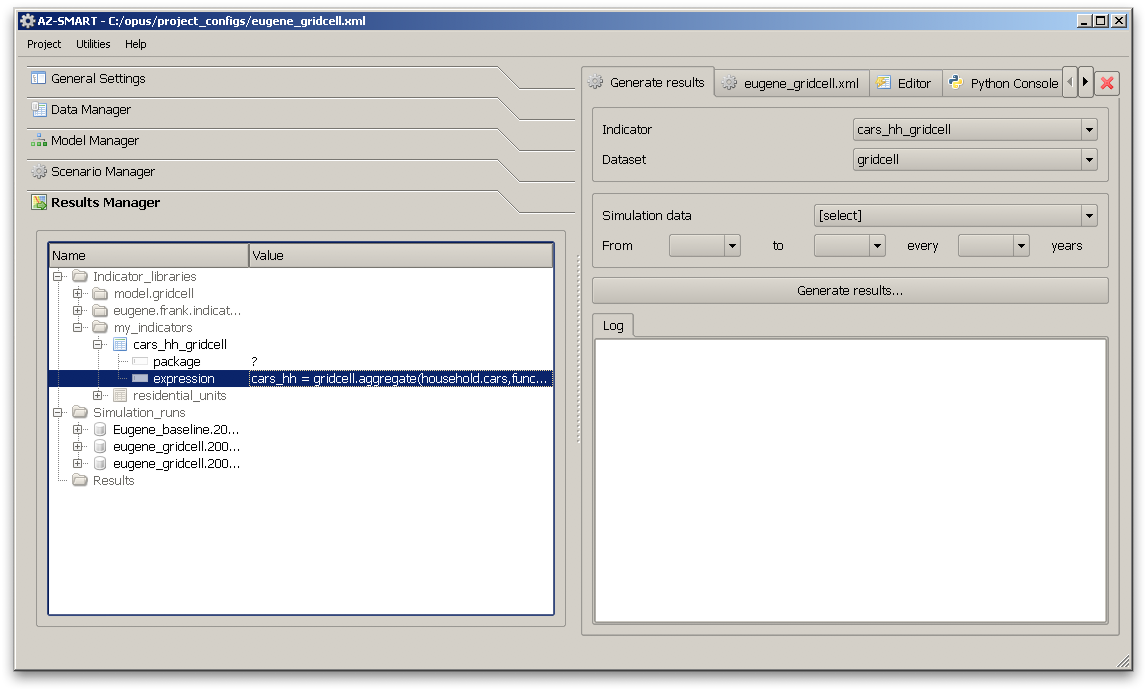
\includegraphics[scale=0.4]{graphics/indicator-cars-gridcell-1.png}
\end{center}
\caption{Generating the Average Cars per Household in a Gridcell}
\label{fig:indicator-cars-gridcell-1}
\end{figure}

\begin{figure}[htp]
\begin{center}
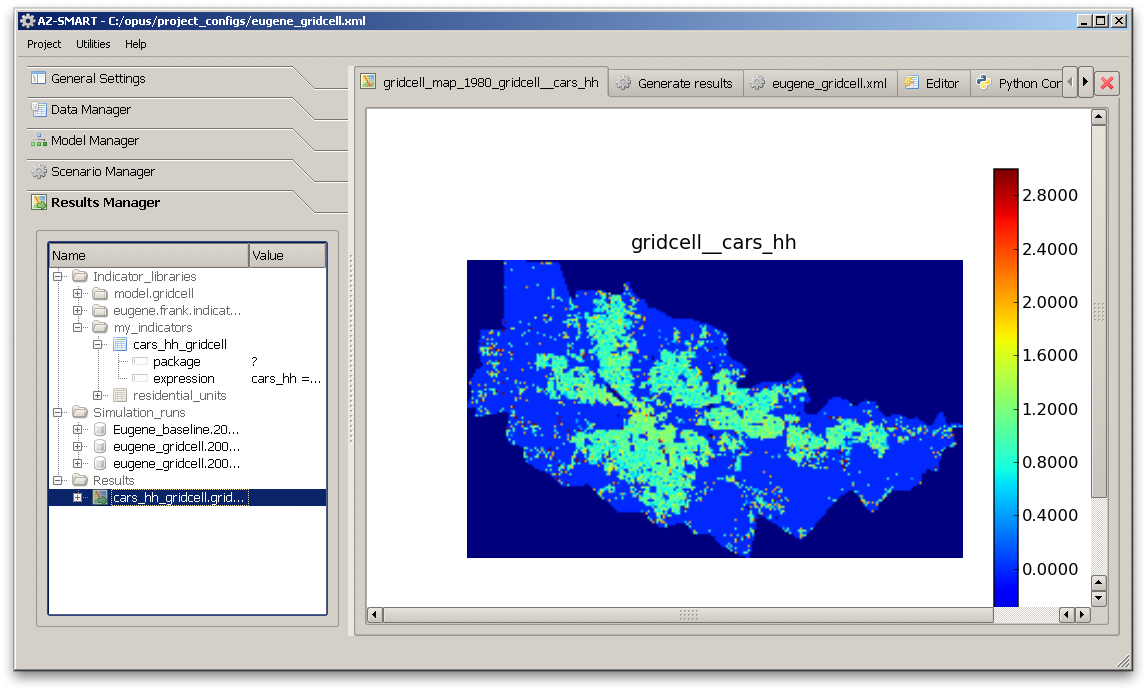
\includegraphics[scale=0.4]{graphics/indicator-cars-gridcell-2.png}
\end{center}
\caption{Generating the Average Cars per Household in a Gridcell}
\label{fig:indicator-cars-gridcell-2}
\end{figure}

In order to compute the second indicator, we will need to average the number of cars per household at the zonal level as follows:

\code{cars\_per\_hh = zone.aggregate(household.cars, intermediates= [gridcell], function=mean)}

The only remaining problem with this is that we cannot display zonal data using Matplotlib, which generates only raster image maps, meaning that it only supports displaying data assigned to gridcells.  Recalling the \verb#disaggregate# function in the expression language, we can just disaggregate the zonal average like this:

\code{cars\_per\_hh = gridcell.disaggregate(zone.aggregate(household.cars, intermediates= [gridcell], function=mean))}

To generate the third indicator of average household size we could use a similar expression:

\code{persons\_per\_hh = zone.aggregate(household.persons, function=mean, intermediates = [gridcell])}

\emph{Unfortunately this zone aggregation will not currently work in the GUI due to some hard coding that assumes indicators added in my\_indicators will be gridcell-based.  This will be fixed shortly.  In the mean time, it would be better to stick to gridcell-based indicators in the my\_indicators section of the Results Manager.}

Now we use a compound expression, to sum the result of two variables, and take the log of the result.  This is to produce the indicator as shown below:

\code{ln\_emp\_pop=ln(urbansim.gridcell.population+urbansim.gridcell.number\_of\_jobs)}

Note that these are variables which can be found on the disk in src/urbansim/gridcell.  The result of visualizing this indicator is shown in Figure \ref{fig:indicator-ln-emp-pop}.

\begin{figure}[htp]
\begin{center}
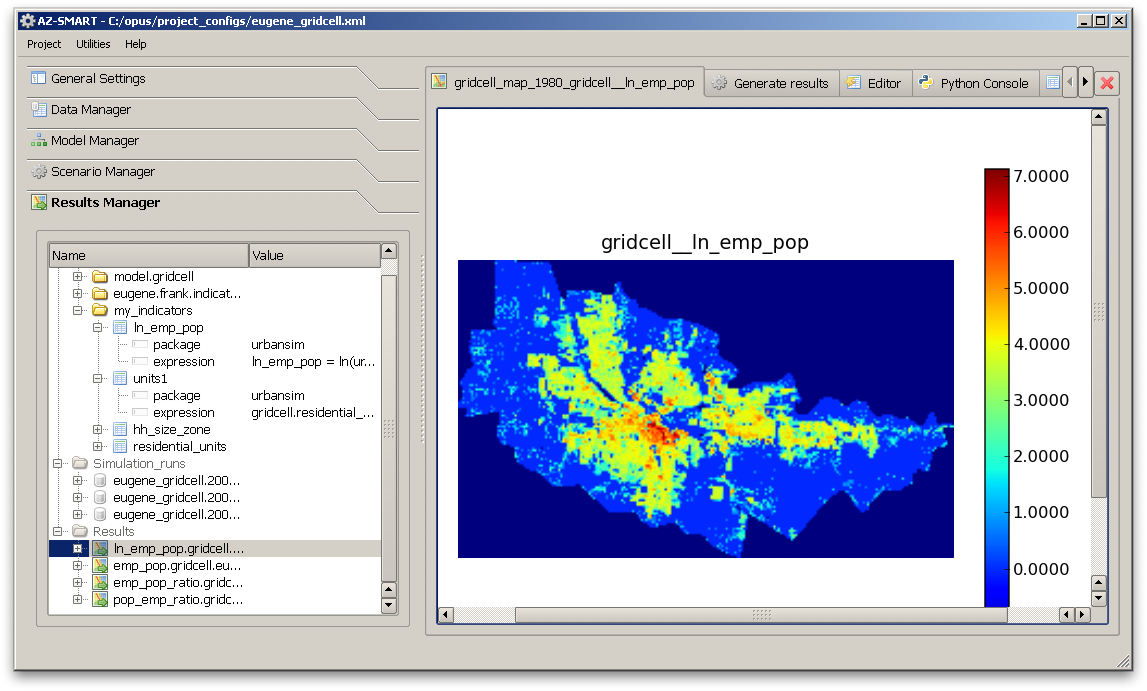
\includegraphics[scale=0.4]{graphics/indicator-ln-emp-pop.png}
\end{center}
\caption{Log of (Population + Employment) by Gridcell}
\label{fig:indicator-ln-emp-pop}
\end{figure}

For the last two indicators in the list to be done, we return to indicators that are already defined in a generic indicator library in the results manager.  To produce the population by zone indicator and visualize it as a table, use the following steps.  Right-click on the population indicators, and select \verb#Generate results with#.  In the form that is created on the right, select the pull-down menu labeled \verb#Dataset# and click on zone.  This is a generalized indicator that uses a simple mechanism to allow different levels of aggregation to be selected in this way, without the need to type in an expression as was done in the preceding examples.  Select a simulation result, and generate the indicator.  Then select the new indicator result containing the indicator values, right-click, and select \verb#View result as# and choose \verb#Table#.  This should generate a browsable table in the form window, as shown below in Figure \ref{fig:indicator-population-zone-table}.

\begin{figure}[htp]
\begin{center}
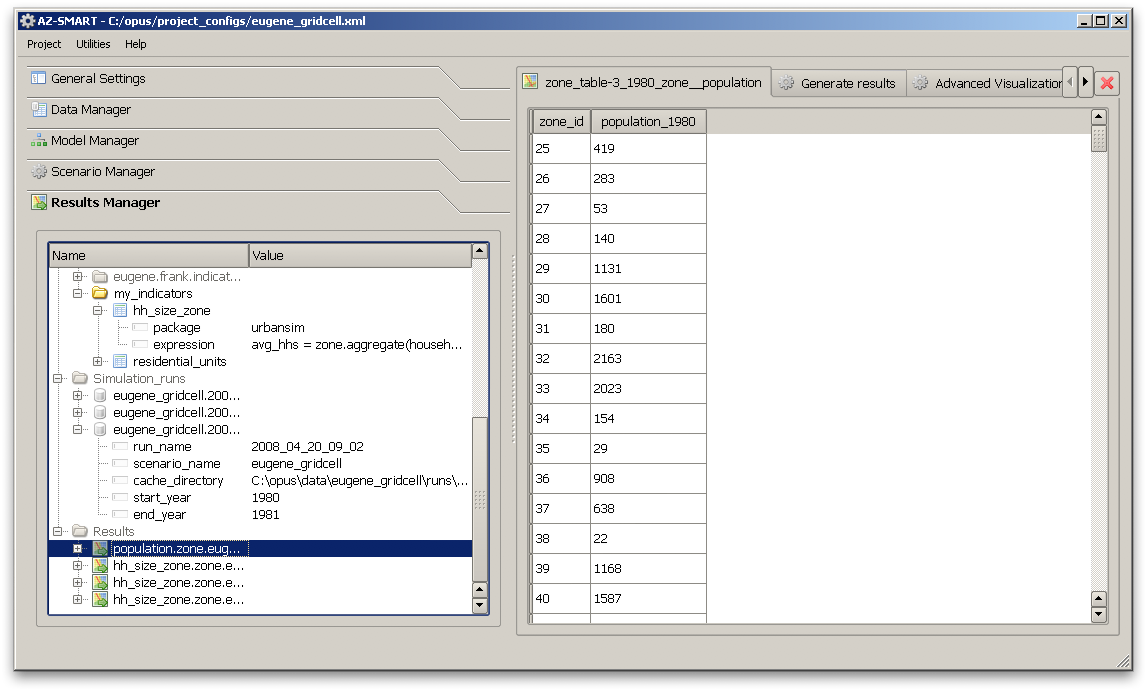
\includegraphics[scale=0.4]{graphics/indicator-population-zone-table.png}
\end{center}
\caption{Viewing the Population by Zone Indicator as a Table}
\label{fig:indicator-population-zone-table}
\end{figure}

Now that we have seen the integrated Matplotlib maps, you might want to know how to export an indicator to a more full-featured GIS system such as ArcGIS (a commercial package from Environmental Systems Research Institute), or PostGIS (an open source package built on the Postgres database).  The Results Manager is now able to export a table with one or more indicators to an ESRI Geodatabase for further analysis and visualization.  In the following example, we export the same indicator result shown above as a table, to an ESRI File-based Geodatabase.  Other Geodatabase formats are also supported.

If the population by zone table result is still available, right-click on the result in the tree on the left-hand side of the window, and select the \verb#View result as# and choose \verb#Advanced visualization#.  It will generate a form as shown in Figure \ref{fig:indicator-population-zone-export}.  We need to add the indicator we have generated to the set, in the upper portion of this form, and select the location of the ESRI geodatabase.  I am assuming that the geodatabase contains a \verb#Feature Class# corresponding to the table being exported. In this example, the table corresponds to the zone feature class.  Once the form is filled in, click on the \verb#Go!# button, to start the export process.  A message will be printed to the log to indicate the completion status of this export process.

\begin{figure}[htp]
\begin{center}
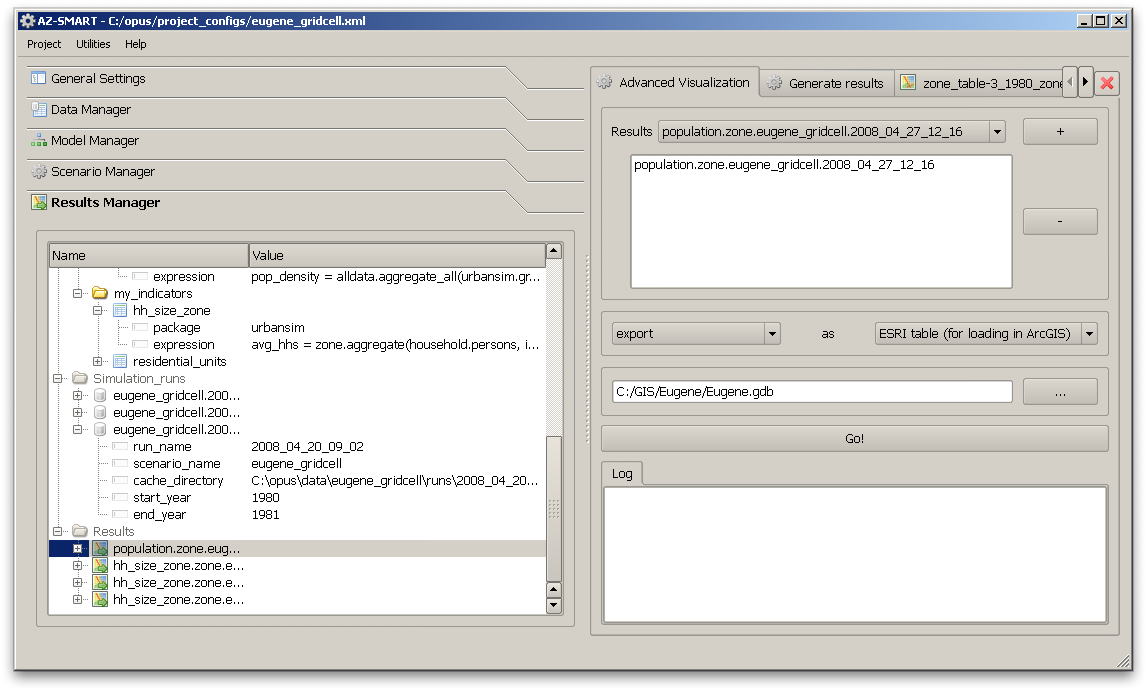
\includegraphics[scale=0.4]{graphics/indicator-population-zone-export.png}
\end{center}
\caption{Exporting the Population by Zone Indicator to an ESRI Geodatabase}
\label{fig:indicator-population-zone-export}
\end{figure}

Once the export is successfully completed, the geodatabase will contain a table that contains the indicator result, with a zone\_id and an ArcGIS \verb#OBJECTID*# that corresponds to the internal object ids in the feature class.  It is safe to join the indicator table result with the feature class using either the objectid or the zone\_id.  The map in Figure \ref{fig:indicator-population-zone-arcgis} shows the result of joining the feature class with the indicator table and generating a thematic map of the populaion by zone, using the zone.acres field to normalize the population, resulting in a map of population density per acre.

\begin{figure}[htp]
\begin{center}
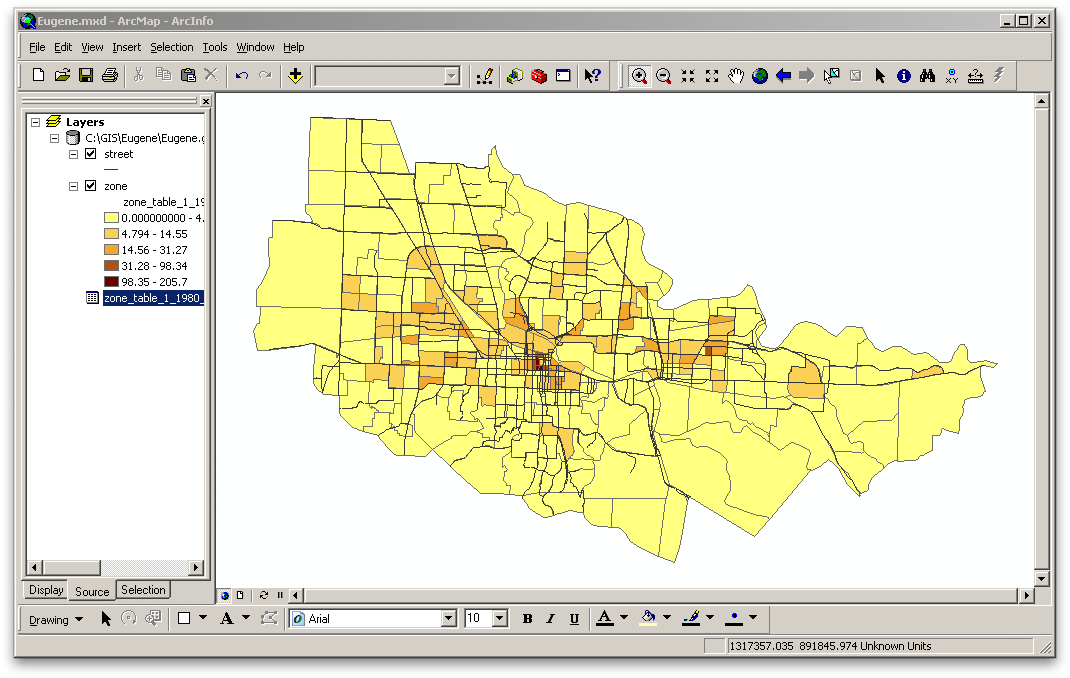
\includegraphics[scale=0.4]{graphics/indicator-population-zone-arcgis.png}
\end{center}
\caption{Mapping the Population by Zone Indicator in ESRI ArcMap}
\label{fig:indicator-population-zone-arcgis}
\end{figure}

\section{(advanced) Creating New Opus Variables}
\label{sec:variables}

Variables in Opus are Python modules containing a single Python \verb#Class# that computes a variable and returns the result.  For demonstration purposes, the population variable in \verb#/src/urbansim/gridcell/population.py# is shown below.  We refer to a variable using a \verb#Pythonpath#, which provides a means for Python to find modules and classes in a directory structure.  So, a reference to this particular module using a \verb#fully qualified path# would be \verb#urbansim.gridcell.population#.  You can find all of the existing variables by browsing on disk in the source code directory.  The directory structure mirrors the parts of the variable name, so that urbansim.gridcell.population is really pointing to /opus/src/urbansim/gridcell/population.py, which is included below as an example.

\begin{lstlisting}
from opus_core.variables.variable import Variable
from urbansim.functions import attribute_label
from variable_functions import my_attribute_label
from opus_core.logger import logger

class population(Variable):
    """Compute the total number of people residing in a gridcell, 
    by summing hh_persons over all households in the gridcell"""
    
    _return_type="int32"
    hh_persons = "persons"

    def dependencies(self):
        return [attribute_label("household", self.hh_persons), 
                attribute_label("household", "grid_id"), 
                my_attribute_label("grid_id")]

    def compute(self, dataset_pool):
        households = dataset_pool.get_dataset('household')
        return self.get_dataset().sum_dataset_over_ids(households, self.hh_persons)


from opus_core.tests import opus_unittest
from opus_core.tests.utils.variable_tester import VariableTester
from numpy import array
class Tests(opus_unittest.OpusTestCase):
    def test_my_inputs(self):
        gridcell_grid_id = array([1, 2, 3])
        #specify an array of 4 hh's, 1st hh's grid_id = 2 (it's in gridcell 2), etc.
        household_grid_id = array([2, 1, 3, 2]) 
        #specify how many people live in each household
        hh_persons = array([10, 5, 20, 30])

        tester = VariableTester(
            __file__,
            package_order=['urbansim'],
            test_data={
                "gridcell":{
                    "grid_id":gridcell_grid_id 
                    }, 
                "household":{ 
                    "household_id":array([1,2,3,4]),
                    "persons":hh_persons, 
                    "grid_id":household_grid_id
                }
            }
        )
        
        should_be = array([5, 40, 20])
        tester.test_is_close_for_family_variable(self, should_be)

if __name__=='__main__':
    opus_unittest.main()
\end{lstlisting}

Some new features presented in this example are the use of a Python Class, which is a topic I will defer for now, the use of dependencies (other variables or primary attributes of datasets that the current variable depends on), and the use of tests in code to ensure that the computation is doing what is expected.  The use of Python modules containing a Class to compute a single variable is flexible and quite powerful, but a bit too complex for most users to use on a regular basis, especially if what is desired is a simple transformation of an attribute or a variable.  Until recently, even something as simple as taking the logarithm of this population variable would have required writing a new module to to that transformation.  Fortunately, this is no longer necessary, since a new Opus Expression language has been implemented.

\chapter{Creating Models in Opus}
\label{chap:creating-models}
\section{Model Types in Opus}

Opus provides infrastructure to develop, specify, estimate,
diagnose and predict with a variety of model types.  The
Opus GUI currently supports the creation of several types of
models by providing templates that can be copied and
configured. More will be added in the future.  These initial
types are:

\squishlist
\item Simple Models
\item Sampling Models
\item Allocation Models
\item Regression Models
\item Choice Models
\item Location Choice Models
\squishend 

\subsection{Simple Models}
%
\label{sec:components-simple-model}
\index{models!opus_core models!simple model}
%
The simplest form of a model in Opus is called, for lack of
imagination, Simple Model.  It is about as simple as a model
can get: compute a variable and write the results to a
dataset.  Here are some examples of what could be done with
a simple model:

\squishlist
\item Aging Model: add one to the age of each person, each
  year
\item Walkability Model: write the result of an expression
  that evaluates the amount of retail activity within
  walking distance
\item Redevelopment Potential Model: compute the ratio of
  improvement to total value for each parcel and write this
  to the parcel dataset \squishend

  A Simple Model template is available in the Model Manager,
  and can be copied and configured in order to create a new
  Simple Model like the examples above. It takes only three
  arguments in its configuration:

\squishlist
\item Dataset: the Opus Dataset that the result will be
  written to
\item Outcome Attribute: the name of the attribute on the
  Dataset that will contain the predicted values
\item Expression: the Opus Expression that computes the
  result to be assigned to the outcome attribute \squishend

\subsection{Sampling Models}
The second type of model template is a Sampling Model.  This
generic model takes a probability (a rate), compares it to a
random number, and if the random number is larger than the
given probability (rate), it assigns the outcome as being
chosen.  Some examples will make the use of this model
clearer. Say we want to build a household evolution model.
We need to deal with aging, which we can do with a Simple
Model.  We also models that predict:

\squishlist
\item Births
\item Deaths
\item Children leaving home as they age
\item Divorces
\item Entering the labor market
\item Retiring
\squishend

For all of these examples -- assuming that we want to base
our predictions on expected rates that vary by person or
household attributes -- we need a more sophisticated model
that we shall call a Sampling Model.  Since we need to
assign a tangible outcome rather than a probability, we use
a sampling method to assign the outcome in proportion to the
probability.  This method is also occasionally referred to
as a Monte Carlo Sampling algorithm.

The algorithm is simple.  Let's say we have a probability of
a coin toss, heads or tails each having a probability of
0.5.  A sampling model to predict an outcome attribute of
Heads, would take the expected probability of a fair coint
toss resulting in an outcome of Heads as being 0.5.  We then
draw a random number from a univariate distribution between
0 and 1, and compare it to the expected probability. If the
random draw is greater than the expected probability, then
we set the choice outcome to Heads.  If it is less than 0.5,
then we set the choice outcome to Tails.  Since we are
drawing from a univariate random distribution between 0 and
1, we would expect that around half of the draws would be
less than 0.5 and half would be greater than this value.
Larger numbers of draws will tend to converge towards the
expected probability by the law of large numbers.  A very
large number of draws should match the expected probability
to a very high degree of precision.

To make the model useful for practical applications, we can
add a means to apply different probabilities to different
subsets of the data.  For example, death rates or birth
rates vary by gender, age, and race/ethnicity, and to some
extent by income.  We might want to stratify our
probabilities by one or more of these attributes, and then
use the sampling model to sample outcomes using the expected
probabilities for each subgroup.

The Sampling Model takes the following arguments:

\squishlist
\item Outcome Dataset: the name of the dataset to receive the predicted values
\item Outcome Attribute: the name of the attribute to contain the predicted outcomes
\item Probability Dataset: the name of the dataset containing the probabilities
\item Probability Attribute: the name of the attribute
  containing the probability values (or rates)
\item List of Classification Attributes: attributes of
  Outcome Dataset that will be used to index different
  Probabilities (e.g. age and income in household
  relocation) \squishend

\subsection{Allocation Models}
%
\label{sec:components-allocation-model}
\index{models!opus_core models!allocation model}
%
Another simple generic model supported in Opus is the
Allocation Model, which does not require estimating model
parameters.  This model proportionately allocates some
aggregate quantity to a smaller unit of analysis using a
weight.  This model could be configured, for example, to
allocate visitor population estimates, military population,
nursing home population, and other quantities to traffic
analysis zones for use in the travel model system.  Or it
could be used to build up a simplistic incremental land use
allocation model (though this would not contain much
behavioral content).

The algorithm for this type of model is quite simple.  To
create an Allocation Model, we need to specify six
arguments:

\squishlist
\item Dataset to contain the new computed variable
\item Name of the new computed variable $Y$, which will be
  indexed by the ids of the dataset it is being allocated
  to, $Y_i$.
\item Dataset containing the total quantity to be allocated
  (this can contain a geographic identifier, and will
  include a year column).
\item Variable containing the control total to be allocated,
  $T$
\item Variable containing the (optional) capacity value $C$,
  indexed as $C_i$
\item Variable containing the weight to use in the
  allocation $w$, indexed as $w_i$, with a sum across all
  $i$ as $W$ \squishend

The algorithm is then just:

\begin{equation}
Y_i = min(round(T\frac{w_i}{W}),C_i)
\end{equation}

If a capacity variable is specified, we add an iterative
loop, from $m$ to $M$, to allocate any excess above the
capacity to other destinations that still have remaining
capacity:

\begin{equation}
T^m = sum(round(T\frac{w_i}{W}) - C_i)
\end{equation}

In each iteration, we exclude alternatives where $Y>=C$, and
repeat the allocation with the remaining unallocated total:

\begin{equation}
Y^m_i = Y^{m-1}_i + (T_m\frac{w_i}{W})
\end{equation}

We then iterate over $m$ until $T^m = 0$ 

This simple algorithm is fairly versatile, and can be used
in two modes: as incremental growth or as total values. If
used in incremental mode, it adds the allocated quantity to
the existing quantities.  The alternative, total, mode for
this model replaces the quantities with the new predicted
values.

\subsection{Regression Models}
%
\label{sec:components-regression-model}
\index{models!opus_core models!regression model}


Regression models are available to address problems in which
the dependent variable is continuous, and a linear equation
can be specified to predict it.  The primary use of this
model in a core model in UrbanSim is the prediction of
property values.  In the context of predicting property
values, the model is referred to as a hedonic regression
\cite{waddell-hedonic-1993}, but the Opus regression model
is general enough to address any standard multiple
regression specification.  Other examples of applications
for this basic class of models would be to predict water or
energy consumption per household, or parking prices.

The basic form is:

\begin{equation}
Y_i = \alpha + \beta X_i + \epsilon_i
\end{equation}

where $X_i$ is a matrix of explanatory, or independent,
variables, and $\beta$ is a vector of estimated parameters.
Opus provides an estimation method using Ordinary Least
Squares, and additional estimation methods are available by
interfacing Opus with the R statistical package.  For the
current discussion, we focus on working with the built-in
estimation capacity.

\subsection{Choice Models}
%
\label{sec:components-choice-model}
\index{models!opus_core models!choice model}
%

Many modeling problems do not have a continuous outcome, or
dependent variable.  It is common to have modeling problems
in which the outcome is the selection of one of a set of
possible discrete outcomes, like which mode to take to work,
or whether to buy or rent a property.  This class of problem
we will refer to as discrete choice situations, and we
develop choice models to address them.

Recall from Section \ref{sec:discrete-choice} that the
standard multinomial logit model
\cite{mcfadden-1974,mcfadden-1981} can be specified as:

\begin{equation}
    P_i = \frac{\mathrm{e}^{V_i}}{\sum_j \mathrm{e}^{V_j}},
\end{equation}
where $j$ is an index over all possible alternatives,
$V_i = \beta\cdot {x}_i$ is a linear-in-parameters
function, $x_i$ is a vector of observed, exogenous, independent
alternative-specific variables that may be interacted with the
characteristics of the agent making the choice,
and $\beta$ is a vector of $k$ coefficients
estimated with the method of maximum likelihood \cite{greene-2002}.

The multinomial logit model is a very robust and widely used
model in practical applications in transportation planning,
marketing, and many other fields.  It is easy to compute and
is therefore fast enough to use on large-scale computational
problems such as residential location choice.  For
explanatory purposes, we will focus initially on choice
problems with small numbers of alternatives, such as the
choice to rent or own a house, or the number of vehicles a
household will choose to own.

Note that there are limitations to the MNL model, and
assumptions a user should be aware of.  The most important
of these is the Independence of Irrelevant Alternatives
(IIA) property, which implies that adding or eliminating an
alternative from a choice set will affect all of the
remaining alternatives proportionately.  Stated another way,
the relative probabilities of any two alternatives will be
unaffected by adding or removing another alternative.  See
\cite{train-book-2003} for a thorough introduction to
discrete choice modeling using MNL and other choice model
specifications.

We now turn to a tutorial for creating models of some of
these types using the Opus GUI.  In the following sections,
we provide a worked example of creating a new model of each
type.  The other model types follow the same pattern in the
Opus GUI.


\section{Interactive Estimation and Diagnostics}
\label{sec:components-model-estimation}
{\bf Please note:} the seattle\_parcel sample data used in the following
description is only to demonstrate functionality.  One should not read too
much into the results, since seattle\_parcel is a small subset taken from
the PSRC project datasets to make its size more manageable.  In particular,
estimating models with certain specifications may give peculiar results,
such as SE and t-values equal to \verb|-1.#IND| or \verb|-1.#INF| due to
an insufficient number of observations, collinearity, or outliers in the
data.  Estimation results that include erroneous results such as these
cannot saved or exported to a sql database, or viewed in the OPUS GUI\@.

\subsection{Estimation of a Regression Model}

In this section, we take up the topic of estimating and diagnosing models
interactively, from the command line.  Eventually the functions described
here will be available in the Graphical User Interface, but as of now they
are only available from the interactive command mode.

Assume we want to estimate the real estate price model in the
seattle\_parcel project, which includes submodels to separately specify the
model for each general land use type.  If you are using a computer with the
Windows operating system, open a command shell, and type the following:

\begin{verbatim}
python -i c:\opus\src\urbansim\tools\start_estimation.py 
-x c:\opus\project_configs\seattle_parcel_default.xml -m real_estate_price_model
\end{verbatim}
(Put this command in one single line or with proper continuation
mark for respective operation system.)

Note that this assumes that your Opus packages are installed in the directory \verb|c:\opus|. 
Also note that the argument of the \verb|-x| option must be given as an absolute path.  

Depending on exactly what the specification is, the result of the call 
would look something like the listing below:
\\

\begin{verbatim}
(clipped results)
...
    ===============================================

    Estimate regression for submodel 28
    Number of observations: 1155
    R-Squared:             0.00277863388614
    Adjusted R-Squared:    0.0010473467922
    Suggested |t-value| >  2.6555330205
    -----------------------------------------------
    Coeff_names	estimate	SE	t-values
       constant	 3.44533	0.307501	 11.2043
       lnempden	0.0281543	0.0176717	 1.59318
      lngcdacbd	 0.15989	0.0943748	 1.69421
    ===============================================

    Estimate regression for submodel 30
    Number of observations: 456
    R-Squared:             0.0678509575502
    Adjusted R-Squared:    0.0595835602779
    Suggested |t-value| >  2.47436715334
    -----------------------------------------------
    Coeff_names	estimate	SE	t-values
       constant	 5.11381	0.300789	 17.0014
     hbwavgtmda	-0.0317135	0.0170671	-1.85817
     ln_bldgage	-0.0357089	0.0241143	-1.48082
      lnemp20tw	-0.0332016	0.0194084	-1.71068
        lnunits	0.0773904	0.0249748	 3.09874
    ===============================================

    Estimating Real Estate Price Model (from urbansim.models.real_estate_price_model): 
    completed...3.2 sec
\end{verbatim}

Since the model was estimated in interactive mode, using the
-i option in the python command to start the estimation, the
program remains active after estimation is completed, and
additional commands may be directly entered at the python
prompt: $>>>$.  Assume that we want to further explore the
data in submodel 30 (mixed-use properties).

One of the first things one might wish to do is to examine
the correlation among the variables in a model.  We can do
this by using one of the built-in estimator methods,
plot\_correlation, with the following command:

\begin{verbatim}
>>> estimator.plot_correlation(30)
\end{verbatim}

The method computes a correlation matrix for the data used
in submodel 30 and generates a plot of this correlation, as
shown in Figure \ref{fig:correlation30}:

\begin{figure}[htp]
\begin{center}
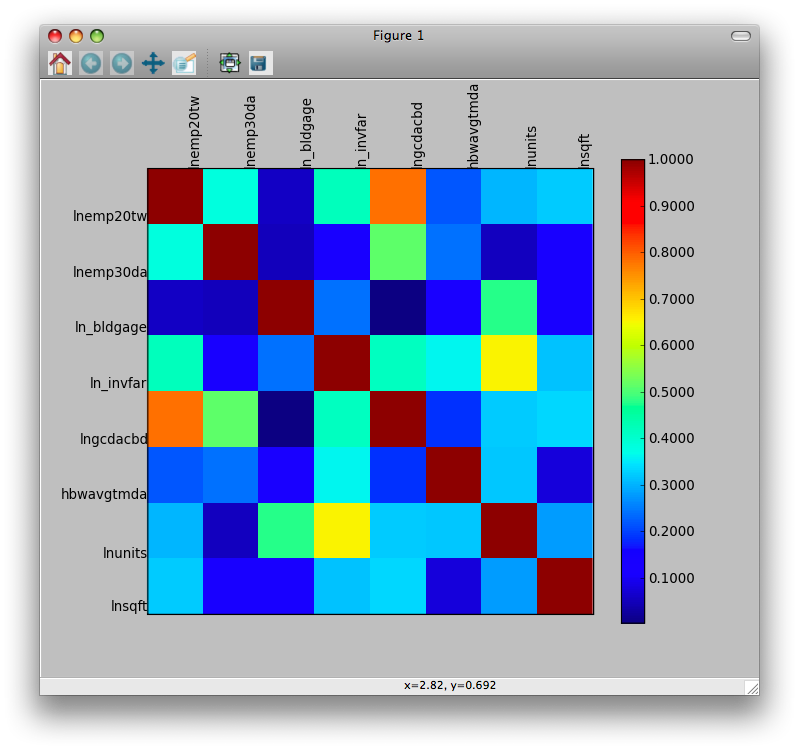
\includegraphics[scale=0.35]{graphics/correlation30.png}
\end{center}
\caption{Correlation Matrix Plot for Submodel 30 in Real Estate Price Modell}
\label{fig:correlation30}
\end{figure}

Note that when a plot is generated from the command line in
Python, control of Python is focused on the graphics window,
and there is no Python prompt available.  When finished
viewing the figure, exit the graphics window by clicking on
the x to close it, and the Python prompt will return for
more interactive commands.

We can retrieve the data for submodel 30 as a dataset that
we can further analyze using Opus methods for the Dataset
class.  Begin with the following command to retrieve the
data and assign it to an object called ds30 (for submodel
30):

\begin{verbatim}
>>> ds30 = estimator.get_data_as_dataset(30)
\end{verbatim}

The syntax above indicates that we are executing a method
called get\_data\_as\_dataset of the class estimator, which
is the class that is running the estimation of the model.
The value 30 in parentheses is an argument being passed to
this method, to identify that we want to retrieve only the
subset of the data that corresponds with submodel 30.  If we
wanted all the data, we would leave out the argument, but
keep the empty parentheses.  Note that nothing special
happens when this command is executed.  If it succeeded, it
will create the new dataset object called ds30, and return
to the python prompt.  At this point, we can use a variety
of built in methods for the dataset class to further explore
the data.  The first of these methods is summary(), which
computes a statistical summary of the data in this object,
like so:
\\

\begin{verbatim}
>>> ds30.summary()
Attribute name	    mean	      sd	      sum	    min	    max
-------------------------------------------------------------------
 lnemp20tw	    8.94	    1.61	  4075.61	5.02388		12.2689
hbwavgtmda	   13.15	     1.8	  5995.99	10.1786		18.0341
   lnunits	    1.08	    1.47	  492.089	      0		5.63121
ln_bldgage	    3.08	    1.41	  1404.12 -0.287682		4.60517

Size: 456 records
identifiers:
  id in range 1-456
\end{verbatim}


Another useful Dataset method is the plot\_histogram, which
computes a histogram for an attribute of a dataset and plots
it, as shown in Figure \ref{fig:histogram-lnsqft}:
\\

\begin{verbatim}
>>> ds30.plot_histogram('ln_bldgage')
\end{verbatim}

\begin{figure}[htp]
\begin{center}
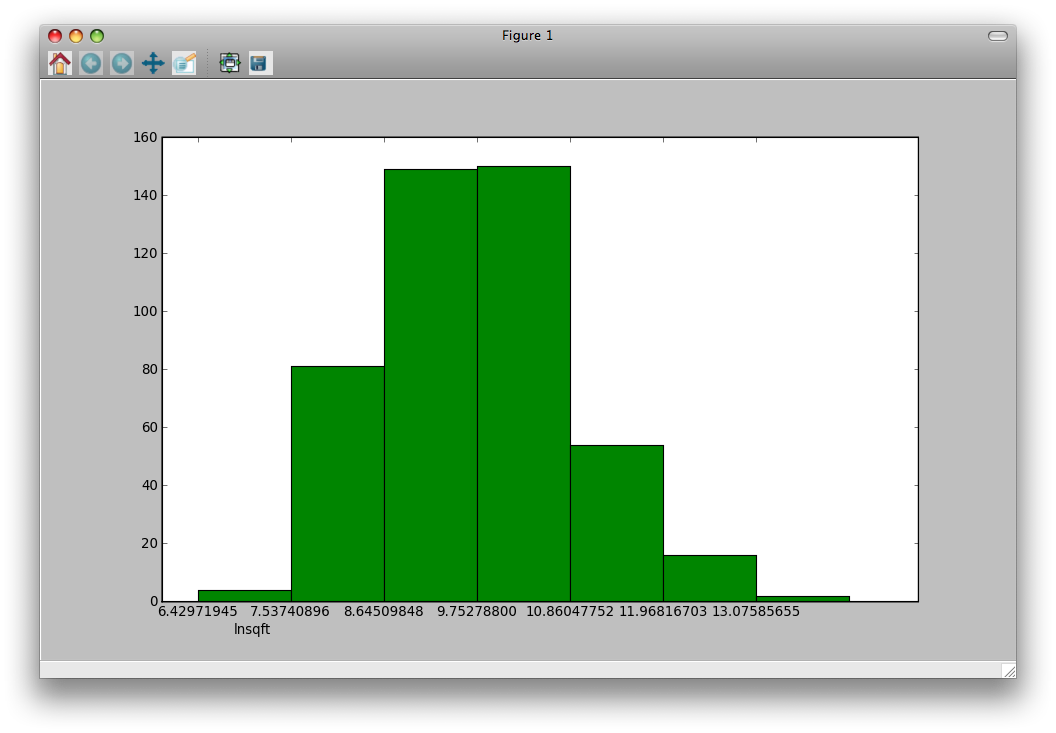
\includegraphics[scale=0.35]{graphics/histogram-lnsqft.png}
\end{center}
\caption{Histogram of Lnsqft from Data in Submodel 30 of the Real Estate Price Modell}
\label{fig:histogram-lnsqft}
\end{figure}

After interactive exploration of the data used in the model,
we might choose to drop or add variables from the
specification.  For demonstration purposes, drop lnemp30da
from the specification of submodel 30, in the GUI, and save
the project.  Alternatively this could be done by editing
the seattle\_parcel.xml (be careful to use an editor that
will not damage the format of the file, for example in
Windows you can use a Notepad version that has added XML
support). Once the specification has been edited and saved,
re-run the estimation for only submodel 30 like this:
\\

\begin{verbatim}
>>> estimator.reestimate(30)
Estimating Real Estate Price Model (from urbansim.models.real_estate_price_model): 
started on Thu May 22 09:36:12 2008
    Estimate regression for submodel 30
    Number of observations: 456
    WARNING: Estimation may led to singularities. Results may be not correct.
    R-Squared:             0.23563241597137002
    Adjusted R-Squared:    0.22368917247092268
    Suggested |t-value| >  2.4743671533372704
    -----------------------------------------------
    Coeff_names estimate        SE      t-values
      constant   7.69055         0.83843         9.17256
    hbwavgtmda  -0.0395769      0.0164105       -2.41168
    ln_bldgage  -0.0340862      0.0220738       -1.54419
     ln_invfar   0.26758        0.0346613        7.71983
     lnemp20tw  -0.030372       0.0279526       -1.08655
     lngcdacbd  -0.545171       0.200477        -2.71937
        lnsqft  -0.118709       0.0256177       -4.63389
       lnunits  0.204933        0.0268876        7.62182
    ===============================================

Estimating Real Estate Price Model (from urbansim.models.real_estate_price_model): 
completed...0.1 sec
\end{verbatim}

Notice that now we see a warning, indicating a problem in
the specification.  Let's drop the least significant
variable, lnemp20tw, and try estimating again:

\begin{verbatim}
>>> estimator.reestimate(30)
Estimating Real Estate Price Model (from urbansim.models.real_estate_price_model): 
started on Thu May 22 09:43:26 2008
    Estimate regression for submodel 30
    Number of observations: 456
    R-Squared:             0.23361810689099238
    Adjusted R-Squared:    0.22337692346414595
    Suggested |t-value| >  2.4743671533372704
    -----------------------------------------------
    Coeff_names estimate        SE      t-values
      constant   6.99788        0.544696         12.8473
    hbwavgtmda  -0.0378939      0.0163405       -2.31901
    ln_bldgage  -0.037881       0.0218001       -1.73765
     ln_invfar  0.271372        0.0344921        7.86765
     lngcdacbd  -0.390517       0.141209        -2.76553
        lnsqft  -0.121596       0.0254847       -4.77133
       lnunits  0.203752        0.0268711        7.58258
    ===============================================
\end{verbatim}

Now the results do not indicate a warning, though we could
experiment further to refine the specification. This
interactive approach is very efficient for rapidly
experimenting with model specifications and re-estimating a
single model.  The same approach is available to estimate a
subset of the models, using the following syntax:

\begin{verbatim}
>>> estimator.reestimate(submodels=[3,7,9])
\end{verbatim}

\subsection{Estimation of a Choice Model}

From the command shell (but not in python), we can also
start the estimation of a choice model, like the housing
type choice model created earlier in this chapter:

\begin{verbatim}
python -i c:\opus\src\urbansim\tools\start_estimation.py 
-x c:\opus\project_configs\seattle_parcel.xml -m housing_type_choice_model 
\end{verbatim}
(Put this command in one single line or with proper continuation
mark for respective operation system.)

The resulting output is shown below:

\begin{verbatim}
(clipped listing)
...
Estimating Choice Model (from opus_core.choice_model): started on Thu May 22 09:51:57 2008
    single_family=(household.disaggregate(building.building_type_id)==19)+1....0.3 sec
    submodel: -2
    Convergence achieved.
    Akaike's Information Criterion (AIC):  333880.22475104179
    Number of Iterations:  18
    ***********************************************
    Log-likelihood is:            -166938.1123755209
    Null Log-likelihood is:       -177492.11908410664
    Likelihood ratio index:       0.059461832801627756
    Adj. likelihood ratio index:  0.059450564695695318
    Number of observations:       256067
    Suggested |t-value| >         3.5289083875852207
    Convergence statistic is:     0.00048567907076085262
    -----------------------------------------------
    Coeff_names     estimate        std err         t-values
      constant      0.600053        0.00561164        106.93
        income      1.13913e-05     5.77362e-08      197.299
    ***********************************************
    Elapsed time:  11.355681 seconds
Estimating Choice Model (from opus_core.choice_model): completed...12.5 sec
\end{verbatim}

Note that the same method used for the regression model,
get\_data\_as\_dataset, can be used to retrieve the data and
analyze it interactively.

There are additional tools in the estimator provides help
for exploring and analyzing the data and model:
\begin{itemize}
%\item plot_choice_set
%\begin{verbatim}
%## plot the alternatives, and its attribute in the alternative set 
%>>> estimator.plot_choice_set()
%>>> estimator.plot_choice_set_attribute('ln(gridcell.residential_units)')
%\end{verbatim}
\item plot_utility helps reveal the relative influence of
  each variable on the utility of the choice model. After
  replacing the estimation procedure of the choice model
  ``bhhh_mnl_estimation'' with
  ``bhhh_mnl_estimation_with_diagnose'' in the
  configuration, enter the interactive estimation mode as
  shown above, then in the Python shell
\begin{verbatim}
>>> estimator.plot_utility()
\end{verbatim}
\item prediction_success_table provides a way to do
  in-sample validation, by applying the estimated
  coefficients to the estimate data to get predicted choices
  and comparing these choices to the observed ones.
\begin{verbatim}
>>> estimator.create_prediction_success_table()
\end{verbatim}
  For location choice model, for example, Household Location
  Choice Model, where there are too many alternatives for
  this to be useful, a summary topology can be provided:
\begin{verbatim}
>>> estimator.create_prediction_success_table(summarize_by= \
    "building_type_id=building.building_type_id")
>>> estimator.create_prediction_success_table(summarize_by= \
    "large_area_id = household.disaggregate(faz.large_area_id, \
    intermediates = [zone, parcel, building])")
# log output to a tab delimited file
>>> estimator.create_prediction_success_table(summarize_by= \
    "area_type_id=building.disaggregate(zone.area_type_id, \
    intermediates=[parcel])",log_to_file='a.out')
\end{verbatim}

\end{itemize}
%% Copyright (c) 2005-2008 Center for Urban Simulation and Policy Analysis,
% University of Washington.  Permission is granted to copy, distribute and/or
% modify this document under the terms of the GNU Free Documentation License,
% Version 1.2 or any later version published by the Free Software Foundation;
% with no Invariant Sections, no Front-Cover Texts, and no Back-Cover Texts.
% A copy of the license is included in the section entitled "GNU Free
% Documentation License".

\chapter{Using the UrbanSim System}
\label{chapter:using-urbansim}
%
The latest incarnation of UrbanSim, UrbanSim 4, is implemented as a
set of packages in Opus. Package \package{opus_core} provides
general functionality, \package{urbansim} contains everything around
land use models, \modelsindex package \package{opus_emme2} is an
Opus wrapper to the travel model EMME/2.\emmeindex

\section{Running a Simulation}
%
\subsection{Support for Production Runs}
The ``Run Manager'' \runmanagerindex is a set of user functionality
provided by the \file{run_manager} \runmanagerindex directories in
the \package{opus_core} and \package{opus_core.services} packages
provide support for specifying, starting, re-starting, and
processing ``production`` runs. \index{production runs} Such a
system is necessary to deal with the long run times for such a model
\modelsindex system, and the large amount of data each run produces.
A 30-year simulation of the Puget Sound Regional Council's (PSRC)
\psrcindex dataset with their EMME/2 \emmeindex travel model, for
instance, takes about 5 days \index{simulation!run time} to complete
and creates about 14 GB of cache data. \index{cache!size of}
\index{simulation!space used by}  These numbers are for a computer
with dual 3.2 GHz Intel\textregistered{} \intelindex
Xeon\texttrademark{} \xeonindex processors and 4 GB of RAM running
Windows XP Professional. \windowstestindex  The PSCS dataset
\datasetindex contains about 800,000 gridcells, 1.3 million
households, and 1.8 million jobs in the initial year. Each UrbanSim
year takes about 1.5 hours to simulate, and each travel model run,
done every 5 years, takes around 12 hours to simulate.

Here are some of the things Run Manager \runmanagerindex helps us do:
\begin{itemize}
  \item Define a run configuration, including what models \modelsindex to run, what years to
  run, etc.
  \item Start a production run.
  \item Monitor the status of all production runs.
  \item Re-start a production run when something goes wrong.
  \item Compute indicators on the results of a production run, including runs
  that are still simulating.
  \item Inspecting specific dataset values from any year of the simulation,
  as when diagnosing problems.
  \item Manage consistency regarding the availability and status of production runs.
\end{itemize}

\subsection{Run Management}
\label{sec:run-manager}
%
Opus contains a set of scripts that simplify the
process of starting and restarting a set of simulation runs.

At the moment, these scripts are a set of command line applications, or tools, in the
\file{opus_core/tools} directory.  They use a database as the central
repository for coordination and context infomation for run managment, by
default called \verb|services|.  If you don't have this database, create it
(you need to do this from within the \file{opus_core/tools}
directory):
\pythonindex
\begin{verbatim}
python create_services_database.py
\end{verbatim}
This creates the database named \verb|services| on the \verb|localhost|
database server using the user name and password specified in the
\verb|MYSQLUSERNAME| \mysqlusernameindex and \verb|MYSQLPASSWORD| \mysqlpasswordindex environment variables. \environmentvariablesindex To use a
different host for the database server, include the \verb|--hostname|
option. To use a different database name, include the \verb|--database|
option:
\pythonindex
\begin{verbatim}
python create_services_database.py --hostname myhost.mydomain --database
myservices
\end{verbatim}

All scripts described below print a help message when called with the
\verb|-h| or \verb|--help| option.

\subsubsection{Start a simulation using a Python Dictionary Configuration}
\index{start a simulation}

The configuration for a simulation is specified by a configuration object.
Previously, a configuration was specified as a Python dictionary, and we
describe the older option in this section.  We are transitioning toward
specifying configurations using an xml project file for use with the Opus
GUI--- see Section \ref{sec:start-simulation-xml} for information on
starting a simulation using an xml configuration but still from the command
line.  In both cases, the configuration is used to specify different parts
of the simulation, such as the years in which to run UrbanSim, what
UrbanSim models \modelsindex to run each year, what types of development
projects exist, how to configure each type of development project,
etc. See, for instance, the run configuration in
\verb|seattle_parcel/configs/baseline.py| (Python dictionary version) or
\verb|seattle_parcel/configs/seattle_parcel.xml| (xml version).

To use the dictionary version of a configuration, the start_run tool
requires that the referenced configuration Python module either (a) defines
a class (e.g. SubsetConfiguration) in a file whose name is
subset_configuration.py, or (b) defines a run_configuration object that is
the configuration object.  In the first case, the class name is the
CamelCase version of the lowercase_with_underscores file name.  \emph{(The
  preferred method is to define a class.)}

To start a simulation using a dictionary-based configuration, use the
script \verb|start_run| with the desired configuration.  First change to 
the directory \verb|opus_core/tools| and execute:
\begin{verbatim}
python start_run.py -c psrc.configs.subset_configuration
\end{verbatim}

Note that the configuration here is specified as it would be in a Python
``import'' statement.

If the \verb|services| database was created using the \verb|--hostname| and/or
\verb|--database| option, you will need to include these options in
\file{start_run.py} as well.  Use the \verb|--help| option to see
\verb|start_run|'s possible command line parameters.

The \verb|creating_baseyear_cache_configuration| entry in the configuration
contains the information specifying the location of the baseyear inputs.  
If \verb|cache_from_mysql| is \verb|True|, the inputs are taken from
the MySQL database specified in the \verb|input_configuration| entry. 
Otherwise, the inputs are taken from the baseyear cache specified in the
\verb|baseyear_cache| entry.  When the inputs are taken from MySQL, they are
used to create a baseyear cache stored in the directory specified by the
\verb|cache_directory| entry, or, if that entry is missing, from an directory
whose name encodes the date-time of the simulation request and is created in the
directory specified by the \verb|cache_directory_root| entry.  

For large amount of data, copying from MySQL to a baseyear cache takes much
longer than creating a new baseyear cache from an existing baseyear cache.  

Option \verb|--directory-to-cache| \index{cache!getting input from existing cache}
can be used to turn off the caching. It takes as argument the directory name
from which data are copied to the new basyear cache \baseyearcacheindex. With
the option \verb|--years-to-cache| one can control specific years to be
copied. The option takes as argument any python \pythonindex expression that returns a list
of years. These two options overwrite entries in the configuration that control
this behaviour.

\subsubsection{Start a simulation using an XML Configuration}
\label{sec:start-simulation-xml}

To start a simulation using an xml configuration from the command line, use
the script \verb|start_run| with the desired configuration.  Change to the
directory that holds the Opus source code and execute:
\begin{verbatim}
python opus_core/tools/start_run.py -x seattle_parcel/configs/seattle_parcel.xml 
       -s Seattle_baseline
\end{verbatim}
(typed all on one line).

Notice that the \verb|-x| option takes a path to the file with the xml
configuration.  Since xml configurations can hold multiple scenarios, the
scenario name must also be specified using the \verb|-s| option.

This same xml configuration can also be used with the Opus GUI ---
documentation on the GUI is forthcoming.

\subsubsection{Restart a simulation}
\index{restart a simulation}
If you halt a run or it fails, you can restart it at the beginning of any year.
To restart the run with \verb|run_id| 42 at the beginning of year 2005, do:
\pythonindex
\begin{verbatim}
python restart_run.py 42 2005
\end{verbatim}
Again, options \verb|--hostname| and \verb|--database| must be included
if non-default values are used.  Note that the above command will delete any
simulation cache \simulationcacheindex directories for years 2005 onward, since
this information is no longer valid once the simulation is restarted at the
beginning of 2005.

If the 2005 travel model failed and you want to restart in 2005 but not re-run
the UrbanSim models, \modelsindex use the \verb|--skip-urbansim| option:
\pythonindex
\begin{verbatim}
python restart_run.py 42 2005 --skip-urbansim
\end{verbatim}

If the 2005 travel model succeeded, and thus wrote its output to the 2006
simulation cache \simulationcacheindex directory, but you need to restart in year 2006, use the
\verb|--skip-cache-cleanup| option:
\pythonindex
\begin{verbatim}
python restart_run.py 42 2006 --skip-cache-cleanup
\end{verbatim}

\subsubsection{Create Baseyear Cache}
\label{sec:run-manager-baseyearcache}
%
One can explicitely create a baseyear
cache \baseyearcacheindex\index{cache!getting input from existing cache} from
the base year database which can be then used for simulation runs. The script
needs a configuration module passed as an argument. The services database is
not used by the script. If the desired module is located at
\file{psrc/configs/subset_configuration.py} under one of the paths found in the
PYTHONPATH \pythonpathindex environment variable, \environmentvariablesindex the command
\pythonindex
\begin{verbatim}
python create_baseyear_cache.py psrc.configs.subset_configuration
\end{verbatim}
caches the database defined in the \verb|subset_configuration| configuration into a basyear
cache. \baseyearcacheindex The \file{create_baseyear_cache} file is located in
the \file{opus_core/tools/} directory, and the above command should be
run from the same directory. An option \verb|--cache-directory|
can be used to pass the directory to be cached into. Alternatively, this can be
specified in the configuration as an entry \verb|'cache_directory'|. See also
Section~\ref{sec:configuration} for configuration and cache control options.

\subsection{What Happens When Running a Simulation?}
\label{sec:run-manager-tasks}
Here are the steps that occur when you start a run via the \verb|start_run|
script:

\begin{itemize}
  
\item \index{cache!unrolling development_event_history}\index{Unrolling 
development_event_history}\index{development_event_history!unrolling} If 
required, it copies all of the tables from the baseyear database specified by 
the configuration into the baseyear cache \baseyearcacheindex and then creates a
set of pre-baseyear \verb|gridcells| tables by unrolling the
\verb|develoment_event_history| data.

The unrolling processes all records in the \verb|development_event_history| 
table.  It starts with the most current year of records, and moves backward in 
time.  For this description, assume that the baseyear is 2000.  The unrolling 
process first loads the gridcell dataset for year 2000.  For each 
\verb|develoment_event_history| record with \verb|scheduled_year| for the prior 
year (e.g. for 1999) it substracts from the gridcells any development by that 
event (e.g. \verb|residential_units|).  Values that go negative are set to 
zero.  Once all events for this year have been ``undone'', the unrolling 
process writes the modified gridcell dataset to the prior year, e.g. to 1999. 
This process is repreated for each year with data in 
\verb|develoment_event_history|.

If you only want 10 years of data to be unrolled, only put those years of data
into your \verb|develoment_event_history| table.

\item Alternatively, it copies files from a previously used baseyear cache into
the baseyear cache for the current run (including the

\item It adds a row to the \verb|run_activity| table in the \verb|services|
database, using a new \verb|run_id| value unique to this run. In order to help
match runs with their cache directory, the name of the cache directory begins
with the \verb|run_id| value, e.g. \file{run_342.2006_04_25_09_40}.

\item For each year in the set of years specified in the configuration:
  \begin{itemize}
  \item Stores to the cache a pickled version of the configurations for that
  year.
  \item Forks a new process to run the set of UrbanSim models \modelsindex for this year.
  The set of models \modelsindex to be run is specified by the configuration. Using a
  separate process helps reduce memory usage, \index{Memory!Using separate
  process} and helps reduce the impact of problems such as memory leaks.  This
  process writes a log file named, e.g., \file{year_2003_log.txt}.
  \item Run the EMME/2 \emmeindex travel model for this year, if specified by the travel
  model's configuration.  The set of steps to run for the travel model is fully
  specified by the \verb|'models'| \modelsindex section of the
  \verb|'travel_model_configuration'|. Typically, it includes a preparation step
  that prepares travel model inputs from the UrbanSim data, a step that
  actually runs the travel model, and one or more steps to puts the results of
  the travel model into the \verb|travel_data| dataset for the current year, so
  the data is visible to the UrbanSim models \modelsindex in that and following years.  Each
  model step is done in a separate process.  The log for the running of the
  model is written to a file named, e.g., \file{emme2_2005_log.txt}. \emmeindex
  \end{itemize}
  \item The run activity table includes status information about the run.  If
  the simulation succeeds, it will add another row to the run activity
  indicating it is done.  If the simulation fails, it will add a row indicating
  that.  The run activity also contains a copy of the configuration, which is
  used when restarting a run.
  \item Whenever a row is added to the \verb|run_activity| table, a row is
  either added or updated in the \verb|available_runs| table in the
  \verb|services| database. This table has a single row per run and records the
  row's current state and information.
\end{itemize}

\section{Configurations}
\label{sec:configuration}
%
A run configuration is a specification of what parts to use in the simulation
and how to configure each part.  Parts include the list and order of models \modelsindex to
run, where to get the input values, where to store the output data, what years
to simulate, what tables to store into the UrbanSim baseyear and simulation
caches \baseyearcacheindex\simulationcacheindex, etc. Each of these parts in
turn may be configurable.  The configuration for a travel model, for instance,
may specify which values to use from the land use models, \modelsindex and what travel model
results to extract in order to use them in the land use models. \modelsindex

Configurations are used in many places in Opus.  Typically, they are specified
via a Python \pythonindex dictionary that then is used to create an instance of the
\class{Configuration} class.

\subsection{Run Manager Configuration}
\label{sec:run-manager-configuration}
%

UrbanSim can be started via the ``Run Manager'' \runmanagerindex (see
Section~\ref{sec:run-manager}) which is controlled by a user-defined
configuration. The following code contains a fully specified configuration
that influences behaviour of the run manager. \runmanagerindex Mandatory entries and default
values for optional entries are marked in the comments. The actual values for
the listed entries are only examples.

\emph{Note: we are in the process of splitting the following configuration
information into separate parts.  Once we are done with that refactoring,
we will update the documentation to the new arrangement.}

\mysqlhostnameindex\mysqlpasswordindex\baseyearcacheindex
\begin{verbatim}
from opus_core.configurations.database_configuration import DatabaseConfiguration
from opus_core.configurations.baseyear_cache_configuration \
    import BaseyearCacheConfiguration
    
from urbansim.configurations.creating_baseyear_cache_configuration \
    import CreatingBaseyearCacheConfiguration


run_configuration = {
    'model_system':'urbansim.model_coordinators.model_system', # mandatory
    'description':'baseline with travel model',      # default: 'No description'
    'cache_directory':'d:/urbansim_cache/',	         # mandatory
    'creating_baseyear_cache_configuration': CreatingBaseyearCacheConfiguration(
        # default: 'urbansim_tmp'+random string
        cache_directory_root = 'd:/urbansim_cache',

        # mandatory
        cache_scenario_database = 'urbansim.model_coordinators.cache_scenario_database',

        cache_from_mysql = False, # default: True

        # mandatory if 'cache_from_mysql' is False
        baseyear_cache = BaseyearCacheConfiguration(
            # mandatory for this block
            existing_cache_to_copy = 'd:/urbansim_cache/run_397.2006_05_23_18_21',
            
            # default: all years in 'existing_cache_to_copy'
            years_to_cache = range(1996,2001)
            },

        tables_to_cache = [ # default: []
            'gridcells',
            'households',
            'jobs',
            'zones'
            ]

        tables_to_cache_nchunks = { # default: each table defaults to 1
            'gridcells':2,
            },

        tables_to_copy_to_previous_years = { # default: no copied tables
            'development_type_groups':1996, # table name and year to put it in
            'development_types':1996,
            'development_type_group_definitions':1996,
            'urbansim_constants': 1996,
            },
        ),
\end{verbatim}

% long script split into two parts since it won't fit on one page

\begin{verbatim}
    'input_configuration': DatabaseConfiguration(    # mandatory
        host_name = os.environ['MYSQLHOSTNAME']      # mandatory
        user_name = 'urbansim',                      # mandatory
        password = os.environ['MYSQLPASSWORD'],      # mandatory
        database_name = 'PSRC_2000_baseyear',        # mandatory
        )
    'output_configuration': DatabaseConfiguration(   # default: No output
                                                     #     configuration
        host_name = os.environ['MYSQLHOSTNAME']      # mandatory for this block
        user_name = 'urbansim',                      # mandatory for this block
        password = os.environ['MYSQLPASSWORD'],      # mandatory for this block
        database_name = 'PSRC_2000_output',          # mandatory for this block
        },
    'base_year': 2000,                               # default: read from table
                                                     #     'base_year' in
                                                     #     'db_input_database'
    'years': (2001, 2030),                           # mandatory
}
\end{verbatim}
The \verb|'model_system'| entry is the full Opus path to the model system that
will be used by the run manager to run/estimate a set of models.

The \verb|'cache_scenario_database'| entry is the full Opus path to the class to use to
create a baseyear cache from the baseyear data in the MySQL database.  The
\verb|'urbansim.model_coordinators.cache_scenario_database'| version creates  both the
baseyear cache, and unrolls the gridcell data to populate prior years with the
gridcell dataset (see Section~\ref{sec:run-manager-tasks}).

Entry \verb|'creating_baseyear_cache_configuration'| contains the configuration
for creating the baseyear cache.

Entry \verb|'cache_directory_root'| is the root directory where data should be
cached during processing. The actual cache directory is created by adding
the run number and date-time string to this directory.

The \verb|'input_configuration'| is a DatabaseConfiguration object
that determines the MySQL \mysqlindex database with the base year
data.

Entry \verb|'output_configuration'| is a DatabaseConfiguration
object that determines the MySQL \mysqlindex database into to which
to write any database tables related to the results of the
simulation run.  Now that indicators are computed from the attribute
cache, the output database is only needed if you wish to use the SQL
indicators.  Before starting the simulation, the run manager will
remove any tables in the output_database, so be sure it doesn't
contain information you want to keep.

Entry \verb|'years'| determines for what
years the simulation should run as a tuple with first and last year to run.

By default, the run manager \runmanagerindex caches all tables from the input database into the
binary baseyear cache \baseyearcacheindex on which then the simulation runs. If
only selected tables should be cached, they can be put into
\verb|'tables_to_cache'|. Note that the simulation itself then does not use the
database anymore, all data are retreived from baseyear cache \baseyearcacheindex
and written to the simulation cache \simulationcacheindex.  That means, if the
entry \verb|'tables_to_cache'| is used, the user must ensure that it contains
all tables that are used by the simulation.

If a database table is so large that Python \pythonindex runs out of memory when copying it
to cache, you can reduce memory usage (but increase the time it takes to cache
the data) by increasing the number of ``chunks'' in which the dataset's \datasetindex
attributes are read from the table. \index{Memory management!When caching data
from input store}\index{Memory management!tables_to_cache_nchunks@\texttt{tables_to_cache_nchunks}} By
default, all attributes of a table are read in a single chunk. Setting the
\verb|'tables_to_cache_nchunks'| configuration for a model will tell the caching code
to use that many chunks.  For instance, if a dataset has 11 attributes, setting
\verb|'tables_to_chunk_nchunks'| to 3 will use three chunks loading 4, 4, and 3
attributes, in each chunk.

For big tables, the caching process can be a very time-consuming task. Often
the baseyear cache \baseyearcacheindex is available from previous runs. Thus,
one can set the entry \verb|'cache_from_mysql'| \mysqlindex to False and define the
\verb|'baseyear_cache'| \baseyearcacheindex block. The directory with the already cached data
should be put into the entry \verb|existing_cache_to_copy|. The run manager \runmanagerindex then
copies data from that directory into the baseyear cache \baseyearcacheindex for this run. If you
want to copy only selected years, they can be specified in the entry
\verb|years_to_cache| as a list of those years; by default all years are
copied. Note that this behaviour can be alternatively controlled directly from
the command line (see description of \verb|start_run| in~\ref{sec:run-manager})
which has priority over entries in this configuration.

The \verb|'tables_to_copy_to_previous_years'| entry is used when a
lag variable needs to compute data for before the base year, and that
computation requires some of the "invariant" data that was copied from the
baseyear database into the baseyear cache.  If this is the case, add those
database tables to the list of tables in the configuration's
\verb|'tables_to_copy_to_previous_years'| entry, and indicate the year to which
to copy the tables.  In general, it is safe to copy the tables to the earliest
year created by the unroll gridcell process.  You can determine what this year
is by examining the year directories created in your baseyear cache.
\emph{(Note: we plan to change this to a better design.)}

There are several run manager \runmanagerindex configurations in Opus. See for example the
directory \file{psrc/configs} for configuration of different PSRC \psrcindex runs.

\subsection{Model System Configuration}
\label{sec:model-system-configuration}
%
If one would pass the above configuration to the run manager, \runmanagerindex it would perform
steps as described in Section~\ref{sec:run-manager-tasks}, but no models \modelsindex would
be run. The configuration should in addition contain entries that control what
models, \modelsindex in what order and with what input and output should be run. It
determines the behaviour of the class \class{ModelSystem}. UrbanSim basic
configuration of the model \modelsindex system can be found in the file
\file{urbansim/configs/general_configuration.py} as an example.

The set of models \modelsindex to run is specified by the entry ``models''. \modelsindex It is a list of
user-defined model names. The order in this list also specifies the order in
which they are run. A production run of UrbanSim consists by default of
following models: \modelsindex
\begin{verbatim}
run_configuration['models'] = [
        "prescheduled_events",
        "events_coordinator",
        "residential_land_share_model",
        "land_price_model",
        "development_project_transition_model",
        "residential_development_project_location_choice_model",
        "commercial_development_project_location_choice_model",
        "industrial_development_project_location_choice_model",
        "development_event_transition_model",
        "events_coordinator",
        "residential_land_share_model",
        "household_transition_model",
        "employment_transition_model",
        "household_relocation_model",
        "household_location_choice_model",
        "employment_relocation_model", 
       {"employment_location_choice_model": {"group_members": "_all_"}},
        "distribute_unplaced_jobs_model"
   ]
\end{verbatim}
Note that the list can contain a particular model multiple times if that model should
run multiple times within one year, such as the ``events_coordinator'' or
``residential_land_share_model'' in the above list.

We can also define a situation when the same model should be run on different subsets of 
a dataset, so called model group\index{model group}. Then we can give the names of the group members to be run, or 
just configure the model group to be run on all subsets. This is the case of ``employment_location_choice_model''
in the list above (see Section~\ref{sec:model-controller-configuration} for further details).
 
By default, the \class{ModelSystem} runs the method
\method{run()} of the listed models. \modelsindex Each entry in this model list can be
alternatively a dictionary containing one entry: The name of the entry is the model
name, the value is a list of model methods to be processed. Thus, one can combine
estimation and simulation of different models. \modelsindex

In addition (or alternatively), the configuration can contain an entry
``models_in_year''. \modelsindex It is a dictionary where keys are years. Each value is
expected to be such list of models \modelsindex as above. In each year, it is checked if
``models_in_year'' \modelsindex (if it is present) contains that year. If it is the case,
its list of models \modelsindex is run, instead of the global set of models. \modelsindex This allows
users to set different set of models \modelsindex for different years, for example an
additional model can be run only in the first year, or last year.

For each entry in the model \modelsindex lists above there must be a corresponding entry in
the ``controller'' configuration which specifies how models \modelsindex are initialized,
what methods to run and what arguments should be passed in. This will be
described in Section~\ref{sec:model-controller-configuration}.

Furthermore, the configuration can contain the following entries (the given
values are defaults set by our system):
\begin{verbatim}
{
    'datasets_to_cache_after_each_model':[],
    'flush_variables': False,
    'seed':0,
    'debuglevel':0
}
\end{verbatim}

The entry \verb|'datasets_to_cache_after_each_model'| specifies names of datasets \datasetindex that
are flushed from memory to simulation cache \simulationcacheindex at the end of each model
run. \index{Memory management!Flushing attributes}\index{Memory management!datasets_to_cache_after_each_model@\texttt{datasets_to_cache_after_each_model}} This reduces the memory
usage, but can increase the run time. We recommend to put datasets in this list
that contain huge amount of data. E.g. UrbanSim sets this entry to ['gridcell',
'household', 'job'].

\verb|'flush_variables'| can further decrease the memory usage. \index{Memory management!flush_variables@\texttt{flush_variables}} If it is True, after each variable
computation all dependent variables are flushed to simulation
cache \simulationcacheindex, regardless to what dataset \datasetindex the variables belong to.
Nevertheless, it increases the run-time considerably.

Entry \verb|'seed'| specifies the seed of the random number generator that is set at
the beginning of each simulated year. It is passed to the \module{numpy} \numpyindex
function \method{seed()} and therefore it should be a tuple with two integer
values. If both values are 0, the function generates a pseudo-random seed
from the current time.

\verb|'debuglevel'| controls the amount of output information.

Models \modelsindex usually need various datasets \datasetindex to run with. They are specified in the
configuration entry \verb|'datasets_to_preload'|. For example,
\begin{verbatim}
{
'datasets_to_preload': {
        'gridcell':{"id_name": "grid_id"},
        'household':{}
}
\end{verbatim}
It is a dictionary that has dataset \datasetindex names as keys. Each value is again a
dictionary with argument-value pairs that are passed to the corresponding
dataset \datasetindex constructor. \class{ModelSystem} \modelsindex creates those datasets \datasetindex at the
beginning of each simulated year and they are accessible to the models \modelsindex
definition in the controller through their names (see
Section~\ref{sec:model-controller-configuration} for details). One should put
here all datasets \datasetindex that will be passed as arguments to the model constructors
or to the model methods to be processed.

If you do not want to make any output to cache, for example in estimation mode, set
\begin{verbatim}
{
    'low_memory_mode': False
}
\end{verbatim}
This should be only used when you're aware what you're doing.
It suppresses any cache writing during the processing (after each model, as
well as at the end of each year) and will not work for a simulation
over multiple years. Also, the memory usage can increase considerably.


\subsection{Models Configuration}
\label{sec:models-configuration}
%
The run configuration can contain an entry \verb|'models_configuration'| \modelsindex which can
include any information specific to models \modelsindex or common to a set of models. \modelsindex The
value of this entry is a dictionary.  Model specific information would be
included in an entry of the same name as the model name used in the entry
\verb|'models'| (see Section~\ref{sec:model-system-configuration}). The
\class{ModelSystem} \modelsindex class makes this information available to the controller
by creating two local variables: \verb|'models_configuration'| \modelsindex (containing the
value of \verb|'models_configuration'| \modelsindex and available to all models) \modelsindex and
\verb|'model_configuration'| \modelsindex (available to each model at the time of its
processing and containing information for this model). See the variable
\verb|'models_configuration'| \modelsindex in the file \file{urbansim/configs/general_configuration.py} for an
example how UrbanSim configures models. \modelsindex

If a model is running out of memory, you can add a \verb|'chunk_specification'|
to that model's configuration. \index{Memory management!Using multiple chunks per model}
\index{Memory management!chunk_specification@\texttt{chunk_specification}} This instructs that model to run in
multiple chunks, each containing a subset of the records (e.g., agents) to
process. This specification can either limit the chunk to contain at most a
given number of records:

\begin{verbatim}
    'chunk_specification':{
        'records_per_chunk':300,     # Put at most 300 records in a chunk
        per chunk },
\end{verbatim}

or specify the number of chunks to use regardless of the number of records:

\begin{verbatim}
    'chunk_specification':{
        'nchunks':10,                # Use 10 chunks
        },
\end{verbatim}

\subsection{Model Controller Configuration}
\label{sec:model-controller-configuration}
%
Each model that is included in the configuration entry \verb|'models'| \modelsindex must have a
controller entry in the \verb|'models_configuration'| \modelsindex entry described in
Section~\ref{sec:models-configuration}.  More specifically, the model specific
section of \verb|'models_configuration'| \modelsindex is expected to contain an entry \verb|'controller'|
for each model. For example, a controller specification for the model
specified by the name \verb|'land_price_model'| would be contained in\\
\verb|run_configuration['models_configuration']['land_price_model']['controller']|.

If a model is specified as a model group \index{model group} it is possible to define a member specific controller, called 
{\em member_name} + '_' + {\em model_name}, e.g. \verb|'home_based_employment_location_choice_model'|.
When choosing the right controller, the \class{ModelSystem} checks for the member specific name. If it is not found,
it uses the group name, in this example \verb|'employment_location_choice_model'|.

The value of this controller entry is a dictionary with a few well-defined entries:
\begin{description}
\item["import"] A dictionary where keys are module names and values are names
  of classes to be imported.
\item["init"] A dictionary with a mandatory entry "name". Its value is the
  name of the class (or class.method) that creates the model. It can be the
  name of the model class itself.  Or, if the model is created via   a
  method e.g. \method{get_model()} of a class \class{MyModelCreator}, it would be
  given as "MyModelCreator().get_model".

  Optional entry "arguments" specifies arguments to be passed into the
  constructor. It is given as a dictionary of argument names and values. All
  values are given as character strings and are later converted by
  \class{ModelSystem} to python \pythonindex objects. If an argument value is suppose to be
  a character string object, it must be given in double quotes, e.g.
  "'my_string'".
\end{description}
If the model in the 'models' entry of the configuration is specified as model group\index{model group}, the controller must contain 
an entry
\begin{description}
\item["group_by_attribute"] Its value is a tuple of a grouping dataset name and grouping attribute (see Sec.~ref{sec:model-group}).
They define the specific kinds of 
subsets of agents on which this model can be run. This dataset must be contained in the 
\verb|datasets_to_preload| entry of the configuration. For example, in the controller of the 
``employment_location_choice_model'' this entry is
\verb|('job_building_type', 'name')|, since the attribute 'name' of the dataset 'job_building_type' contains the various
building types of jobs for which we want to run the model, i.e. 'commercial', 'governmental', 'industrial' and 'home_based'.
If the 'group_members' entry (of the 'models' entry of the configuration) for this model is equal to '_all_', the model runs 
for all values found in this dataset. The  'group_members' can also be a list specifying explicitely for which types the model 
should be run. 
\end{description}

The \class{ModelSystem} class evaluates the given imports and creates an
instance of the model by processing the \verb|'init'| entry. The remaining entries
below are related to specific methods of the created model instance.  As
mentioned in Section~\ref{sec:model-system-configuration}, models \modelsindex
that are listed in the \verb|'models'| entry of the run configuration can be also
specified using a list of methods to be processed. If the list is not given, a
method \method{run()} is assumed to be the only method to be processed. The
\class{ModelSystem} iterates over the set of methods. It first processes a
``preparation'' method (if required) and then the method itself. For this purpose,
the controller should contain the following entries:

\begin{description}
\item['prepare_for_...'], where \verb|...| is the the method
to be processed, e.g. \verb|'prepare_for_run'| is the method to call to prepare
to run. This configuration entry is a dictionary with an
optional entry \verb|'name'| giving the name of the preparation method. If \verb|'name'| is
missing, the method name is assumed to be the same as this entry name. Optional
entry \verb|'arguments'| specifies arguments of this method (see \verb|'arguments'| in \verb|'init'|
above). Optional entry \verb|'output'| defines the name(s) of the output of this
method.  It can be then used as an input to other methods or models. The entry
\verb|'prepare_for...'| is optional and if it's missing, no preparation procedure is
invoked. There can be as many \verb|'prepare_for...'| entries as there are
methods specified.
\item[{\it procedure}] The procedure name must match to the method names given
in \verb|'models'| (there must be one entry per method), or be called \verb|'run'| if no
methods are specified in \verb|'models'|. It is a dictionary with optional arguments
\verb|'arguments'| and \verb|'output'| (see above).
\end{description}

The entry \verb|'arguments'| in the above items can contain any character
strings that are convertable (using python's \verb|eval()|) to python \pythonindex objects,
including python \pythonindex expressions. They must be objects that are known to the
\class{ModelSystem}, for example datasets \datasetindex that are defined in
\verb|'datasets_to_preload'| (described in
Section~\ref{sec:model-system-configuration}), since those are created prior to
the simulation. They can be called either by the dataset \datasetindex name, or using
\code{datasets['{\it name}']}. Also, the \verb|model_configuration| and
\verb|models_configuration| objects described in
Section~\ref{sec:models-configuration} can be used in \verb|'arguments'|. Other
objects that \class{ModelSystem} provides are \verb|sql_storage|
(\class{Storage} object for the input database), \verb|cache_storage|
(\class{Storage} object for the simulation cache \simulationcacheindex storage
in the simulated year), \verb|base_cache_storage| \baseyearcacheindex (\class{Storage} object for
the baseyear cache \baseyearcacheindex storage in the base year),
\verb|model_resources| (all preloaded datasets as an object of
\class{Resources}), \verb|year| (simulated year), \verb|resources|
(Configuration passed into the simulation), \verb|dataset_pool| (object of class \class{DatasetPool} pointing to the current
dataset pool).  If you are using any class names
as arguments, you need to make sure, that those classes are known to the
\class{ModelSystem}, e.g. by putting the appropriate import statement into the
\verb|'import'| section of the controller.

Here is an example of a controller settings for the land price model in UrbanSim:
\modelsindex\datasetindex
\begin{verbatim}
run_configuration['models_configuration']['land_price_model']['controller'] = {
    "import": {"urbansim.models.corrected_land_price_model":
                                                "CorrectedLandPriceModel",
              },
    "init": {"name": "CorrectedLandPriceModel"},
    "prepare_for_run": {
        "arguments": {"specification_storage": "base_cache_storage",
                      "specification_table": "'land_price_model_specification'",
                      "coefficients_storage": "base_cache_storage",
                      "coefficients_table": "'land_price_model_coefficients'"},
        "output": "(specification, coefficients)"
        },
    "run": {
        "arguments": {"n_simulated_years": "year-resources['base_year']",
                      "specification": "specification",
                      "coefficients":"coefficients",
                      "dataset": "gridcell",
                      "data_objects": "datasets" ,
                      "chunk_specification":"{'nchunks':2}"
                     }
           }
   }
\end{verbatim}
Note on an implementation of model group\index{model group}: A constructor of 
a model group, must take as its first argument an object of class \class{ModelGroupMember} (Sec.~\ref{sec:model-group}). 
The controller should though ignore this argument, since the \class{ModelSystem} automatically takes care of creating this object 
and passing it to the model constructor.

\section{Output}
%
\subsection{The Output Database}

The simulation reads and writes all of its data from the simulation cache.  It 
does not directly read or write to any database. 
If you wish to move data from the simulation cache to a MySQL database, use the
\verb|do_export_cache_to_sql_database.py| tool located in
\file{opus_core/tools}. 

\subsection{File-Based
Cache}\label{cache} \baseyearcacheindex\simulationcacheindex

For a variety of reasons, described below, UrbanSim uses two forms of file-based
caches:
\begin{description}
\item[baseyear cache] \baseyearcacheindex
Stores the attribute values read from the baseyear
database.  This includes data for the base year, and data for years before the
base year (unrolled from data in the baseyear).  This data is not modified
during the simulation.

\item[simulation cache] \simulationcacheindex
Stores the attribute values for datasets used during the simulation.
\end{description}
While the distinction between the read-only baseyear cache \baseyearcacheindex and read-write
simulation cache \simulationcacheindex is useful understanding the system, during simulation both
caches form a single cache that UrbanSim datasets \datasetindex and models \modelsindex mine to gather data
for the current and prior years.

\subsubsection{Reasons to Use Cache}
The UrbanSim simulations run on top of a file-based cache.  The initial reason
for the cache was to improve performance, and has turned out to be very useful for
many features:

\begin{itemize}
  \item The cache is much faster to access than the MySQL \mysqlindex database, at least,
  so using the cache dramatically speeds up our processing.
  \item In many cases, a simulation will require more data than can fit in RAM.
  The simulation cache \simulationcacheindex provides a place to store computed
  or non-computed values so that we only need to keep in memory just enough
  data for the computation at hand. \index{Memory management!Caching data}
  \item Lag variables use the baseyear cache \baseyearcacheindex and simulation
  cache \simulationcacheindex to quickly get data from prior years, often
  without having to re-compute it.
  \item When preparing for a simulation, UrbanSim uses the data from lag tables
  (see~\ref{lag-tables}) in the baseyear to create historical data in the
  baseyear cache \baseyearcacheindex for years before the base year.  This
  allows the simulation to run without any distinction between historical and
  predicted data.
  \item Lag variables on gridcell data need gridcell information from prior
  years.  UrbanSim can use the information in the
  \verb|development_event_history| table to create gridcell data for before the
  baseyear by ``unrolling'' the development events from before the base year.
  \item When looking for a primary attribute \primaryattributesindex for a given dataset, \datasetindex Opus
  looks first in the current year.  If the data is not in that year's cache,
  Opus automatically looks backward thru prior years until it finds it.  This
  allows Opus to only store to cache primary attributes \primaryattributesindex in the years in
  which they are modified, while still getting the performance and memory
  improvements by using the cache. \index{Memory management!Caching data}
  \item The information in the simulation cache \simulationcacheindex includes all
  of the intermediate variable values produced for every year.  This allows us
  to inspect inspect this data for diagnostic purposes.
  \item Our indicator framework mines the cache data to produces charts, tables
  and maps that help to diagnose runs as well as providing input to policy
  decisions.
\end{itemize}


\subsubsection{What is Written to Cache}
During a simulation, UrbanSim writes a variety of data to the simulation
cache. \simulationcacheindex These include:
\begin{itemize}
  \item Any dataset \datasetindex attribute read into memory or computed during the year.
  \item A log file for each year, containing anything written to the UrbanSim
  logger.
  \item A log file for the top-level process that runs each year of the
  simulation.
  \item Meta-data about the information in the simulation
  cache, \simulationcacheindex such as the ``version'' of each variable so that
  we only need to recompute variables \variablesindex when their inputs change.
\end{itemize}

You can adjust the frequence with which the simulation flushes dataset \datasetindex
attribute \attributesindex values to the simulation cache: \simulationcacheindex

\begin{itemize}
  \item After computing each year.  This is always done.
  \item After computing each model.  Set
  \verb|'datasets_to_cache_after_each_model'| in the run configuration to
  a list of dataset \datasetindex names you wish to cache. An empty list (default) causes
  no caching.
  \item After computing each variable. \variablesindex Set \verb|'flush_variables'| \variablesindex to \verb|True| in the
  run configuration.
\end{itemize}

\subsubsection{Deleting the File-Based Cache}

The \verb|delete_run| script in \file{opus_core/services/run_manager} directory
provides an easy way to delete cached run data while maintaining the
consistency of the services database.  This is useful, since a simulation can
produce multiple gigabytes of data.

To delete all data for run with \verb|run_id| 42, and remove that run's
information from the \verb|available_runs| table in the \verb|services|
database use:

\pythonindex
\begin{verbatim}
python delete_run.py --run-id 42
\end{verbatim}

To delete a set of years without removing the information from the
\verb|services| database, use the \verb|--years-to-delete| option.  This
option takes an arbitrary Python \pythonindex expression that creates a list of integers.
For instance, to remove the cached data for years 2001 through 2029 use:

\pythonindex
\begin{verbatim}
python delete_run.py --run-id 42 --years-to-delete range(2001,2030)
\end{verbatim}

\section{Converting the Base Year Data}
The base year database for the Opus UrbanSim~4 is almost the same as that used
by UrbanSim~3 (the Java version).  Instructions on converting the database are
available at
\mbox{\url{http://www.urbansim.org/opus/opus_manual/docs/scripts/converting_3_to_4.html}}.

\subsection{Lag Tables}\label{lag-tables}

The baseyear database may contain data from before the base year.  If you want
this data to be available to the simulation, put it into a lag table whose name
is the same as the non-lag table for that dataset except with \verb|_lag| at the
end, e.g. \verb|gridcells_lag|, and that contains a \verb|year| column indicating
the year for each row.  The first step of a simulation run copies this lag
data into the baseyear cache, \baseyearcacheindex so that it can be accessed by lag variables. \variablesindex


%% $Id: indicators.tex,v 1.61 2007/06/01 23:49:22 borning Exp $

% Copyright (c) 2005-2007 Center for Urban Simulation and Policy Analysis,
% University of Washington.  Permission is granted to copy, distribute and/or
% modify this document under the terms of the GNU Free Documentation License,
% Version 1.2 or any later version published by the Free Software Foundation;
% with no Invariant Sections, no Front-Cover Texts, and no Back-Cover Texts.
% A copy of the license is included in the section entitled "GNU Free
% Documentation License".

\chapter{Generating and Visualizing Indicators}
\indicatorsindex

As used in the planning literature, an indicator is a
variable \variablesindex that conveys information on the condition or
trend of an attribute \attributesindex of the system considered.  The
indicator will then have a specific value at a given time.
For UrbanSim, indicators provide the principal mechanism
for presenting simulation results to modelers and other stakeholders so
that they can be assessed and compared.  In addition, modelers use
indicators diagnostically to help assess whether the
system is operating in a reasonable fashion and to help debug problems.

We will often be interested in the value of an indicator at different levels of
aggregation, for example, 
population in each grid cell, in different political divisions of
the region, and for the region as a whole.  We will often also be
interested in the change in the value of an indicator
in successive years, or from each year of the
simulation to the baseyear, or between two different scenarios.
Indicator values should be displayed in an
appropriate way, for example, using graphs,
\index{graphs} tables, \index{tables} or choropleth maps.
\index{maps} Some key indicators for both policy
evaluation and model diagnosis include population, residential
units, land value, employment, and square feet of commercial,
industrial, and governmental space, all at various levels of
aggregation, from the grid cell up.

Requests for indicator visualizations can be made using either a graphical
interface (Section \ref{sec:indicator-configuration-gui}), or a Python
script (Section \ref{sec:indicator-configuration-script}).  The GUI is more
user-friendly, but only allows a single indicator request to be made at a
time.  Scripts are Python code, but one script can specify allow an entire
suite of indicators that is to be computed

There is online documentation for some of the indicators, 
linked from \url{http://www.urbansim.org/opus}.  See Section
\ref{sec:writing-indicators} for information on writing indicator
\indicatorsindex documentation.  (Formerly we computed the values for
indicators using SQL queries, but this proved too slow in many cases, so we
switched to using Opus attributes exclusively.  There was much more
extensive documentation for the SQL versions of the indicators; if there is
demand for this and as time allows, we will also provide documentation for
other indicators represented as Opus attributes.)

\section{Computing the Values of Indicators using Opus Attributes}

The basic class for dealing with data in Opus is the class \class{Dataset}
\datasetindex (Section \ref{sec:opus-core-datasets}).  A dataset
\datasetindex is a collection of attributes \attributesindex for a
particular type of entity, such as a set of grid cells, or a set of
households.  Each member in this set has the same set of characteristics,
such as income of household.  In Opus, these characteristics are called
attributes. \attributesindex Attributes \attributesindex can be either read
from a data store (primary attributes), \primaryattributesindex or computed
using an Opus variable definition (computed
attributes). \computedattributesindex

Any Opus attribute \attributesindex (primary or computed)
\computedattributesindex\primaryattributesindex can be used as an
indicator, \indicatorsindex although of course only some attributes
\attributesindex will be particularly \emph{useful}
indicators. \indicatorsindex The primary attributes \primaryattributesindex
of interest are commonly in the database tables for the given Opus
application.  For UrbanSim, these database tables and their attributes
\attributesindex are documented in Chapter
\ref{chapter:urbansim-database-tables}, ``UrbanSim Database Tables.''  (A
fine point: models or other Opus code can also create other primary
attributes, \primaryattributesindex even on the fly --- so the database
tables don't provide a comprehensive list of primary
attributes. \primaryattributesindex However, probably all of the primary
attributes \primaryattributesindex of interest for indicators
\indicatorsindex will be in the database tables.)  Each computed attribute
\computedattributesindex is defined by an Opus variable \variablesindex
definition.

For both primary \primaryattributesindex and computed attributes,
\computedattributesindex the attribute \attributesindex to be used as an
indicator \indicatorsindex can be identified by its fully-qualified name,
for example:

\begin{itemize}
\tight
\item \module{urbansim.gridcell.residential_units}
\item \module{urbansim.gridcell.population}
\item \module{zone.aggregate(gridcell.residential_units, function=sum)}
\end{itemize}

Of these, the first one (\module{urbansim.gridcell.residential_units}) is a
primary \primaryattributesindex attribute --- the number of residential
units is part of the data stored for each gridcell --- while the other two
are computed. \computedattributesindex (Population is computed, even for
gridcells --- for a gridcell, it is computed by summing the number of
persons in each household located in that grid cell.  Residential units at
the zone level is computed, \computedattributesindex since it is computed
by summing, via the aggregate function, the number of residential units in
each gridcell in that zone.)

Attributes \attributesindex can also be in project-specific packages in
addition to ones in the \package{urbansim} package.  For example, in our
PSRC \psrcindex application of UrbanSim, one of the indicators
\indicatorsindex is
\module{psrc.zone.travel_time_hbw_am_drive_alone_to_cbd}, for the
\verb|zone| geography defined for this application.

As with other Opus variables, \variablesindex the variable \variablesindex
name for variables \variablesindex used as indicators \indicatorsindex can
be a template that matches a family of related variables, \variablesindex
such as \module{psrc.houeshold.has_DDD_cars}.  This variable
\variablesindex can then be instantiated with a particular number of cars,
e.g.\ \module{psrc.houeshold.has_2_cars}.

The values of a set of indicators \indicatorsindex can be computed,
and charts and maps produced for these values, using either a
graphical interface, or programatically (using a Python script).
These two techniques are described in the following two sections
(\ref{sec:indicator-configuration-gui} and
\ref{sec:indicator-configuration-script} respectively).  

\section{The Indicator GUI}
\label{sec:indicator-configuration-gui}

The Indicator GUI is specified using the Enthought Traits packages
(\url{http://www.enthought.com}).  It provides a graphical editor for
specifying and generating an indicator.  The GUI can be started by running
the indicator_gui.py located in the indicators subdirectory of each
project. For example, for the PSRC application, run
\file{psrc/indicators/indicator_gui.py}.  This will open the indicator GUI.

Currently, there are two parts of the GUI: specifying scenario information and 
specifying the indicator. 

\subsection{Specifying Scenario Information}
The scenario specification pane is where you input information 
about which scenario results should be used for computing the indicators. 
The fields are:
\begin{description}

\item[Cache directory] is the directory holding the cache with the
  simulation results from which indicators are to be produced.

\item[Comparison cache directory] is an optional field. It can 
be set to point to another cache directory of simulation results.
If it is specified, the computed indicators will be compared 
between the two scenarios. See section \ref{sec:indicator-cross-scenario} 
for more details. 

\item[Compare to another cache directory] is a checkbox that toggles
on and off the ability to specify a comparison cache directory.

\end{description}

\subsection{Specifying Indicators}
The indicator specification pane is where you specify the 
indicator you wish to compute. There are four possible output 
types: Tab-deliminated Table, Comma-separated Table, Map, and 
Chart. The fields are:

\begin{description}

\item[Type] is the output type of the indicator.

\item[Attribute] is the fully qualified path of an opus variable, as 
described at the beginning of this section. 

\item[Name] is the desired name of the indicator. This field is optional.
It defaults to the attribute field.

\item[Dataset] is the dataset for which the indicator should be 
computed from (e.g. grid cell, zone).

\item[Years] lets you select the years for
which these indicator values should be computed. Examples include
``2001,2003'' and ``2010-2020'', the latter of which results in 
the indicator being computed for all years between 2010 and 2020
inclusive. 

\item[Comparison cache directory] is an optional field. It can 
be set to point to another cache directory of simulation results.
If it is specified, the computed indicators will be compared 
between the two scenarios. See section \ref{sec:indicator-cross-scenario} 
for more details. 

\item[Compare to another cache directory] is a checkbox that toggles
on and off the ability to specify a comparison cache directory.

\end{description}

The \verb|map| visualization type has an additional optional field: 
\begin{description}
\item[Scale] specifies the minimum and maximum values for the map coloring. 
\end{description}  

There is a ``run'' button at the bottom of the GUI that starts the indicator 
computations.  There is also a ``view results'' button that launches a 
static HTML page with the results of the indicator computations in a 
web browser (see section \ref{sec:indicator-results}). In
addition, the ``file'' menu includes items for saving a configuration, and
opening a previously saved one.  (The ``run'' action is also available via
the run menu.) 

\section{Constructing an Indicator Configuration using a Python Script}
\label{sec:indicator-configuration-script}

It is also possible to set up a indicator request configuration
programatically, i.e.\ using a Python script. A full example can be found at 
\module{opus_core.indicator_framework.make_indicators_example}. In this 
section, the elements of setting up an indicator request configuration 
is described. There are three parts: setting up the \verb|SourceData| 
object, generating a list of indicator objects, and running the 
indicators through the \verb|IndicatorFactory|.

\subsection{Constructing the SourceData object}

The first step is to construct a \verb|SourceData| object.
The SourceData specifies 
the location of the simulation results that should be 
used for computing the indicators, the years for which the indicators should be
computed, and, optionally, a second data directory for which the indicators will
be compared against. Each indicator requires a source data object to be passed
to it. Every SourceData object accepts the following arguments:
\begin{description}

\item[dataset_pool_configuration] is an object that handles which 
datasets get loaded and in what order. 

\item[cache_directory] is a path to the directory containing the 
simulation results that the indicators should be computed from.

\item[comparison_cache_directory] is an optional field. Set this field 
to the path to a second cache directory in order to run a 
cross-scenario indicator comparison. See \ref{sec:indicator-cross-scenario}
for more information.

\item[run_description] is a description of this indicator batch. 
This field is optional. 

\item[years] are the default years that all the indicators will be computed for.
This field is optional, although all indicators will then need to have a 
years field if not specified here.

\end{description}

Here is an example:

\begin{verbatim}
source_data = SourceData(
   cache_directory = r'D:\urbansim_cache\run_1090.2006_11_14_12_12',
   comparison_cache_directory = r'D:\urbansim_cache\run_1091.2006_11_14_12_12',
   years = [2010],
   dataset_pool_configuration = DatasetPoolConfiguration(
         package_order=['urbansim','opus_core'],
         package_order_exceptions={},
         ),                  
)
\end{verbatim}

\subsection{Creating Indicator Objects}

The next step is to create a list of indicators to generate. There are a 
number of different visualization types available. 

\begin{description}
\item[\code{table}] \index{tables} produce a table \index{tables} of indicator \indicatorsindex values
\item[\code{chart}] \index{charts} produce a chart \index{charts} or graph \index{graphs} using matplotlib \matplotlibindex
\item[\code{map}] \index{maps} produce a choropleth map \index{maps} using matplotlib \matplotlibindex
\item[\code{dataset_table}] produces a table for every specified year 
with the values of each of the specified indicators.
\end{description}

First, the fields 
that are common to each visualization are described, and then examples and
specific fields are described for each visualization type. Every indicator 
object takes the following parameters:

\begin{description}
\item[source_data] references the desired \verb|SourceData| object (see above). 

\item[dataset_name] is the name of the dataset that this indicator will be 
computed for.

\item[years] are the years that the indicator will be computed for.
This field is optional if the \verb|SourceData| object also 
has a years field. The indicator years field overrides
the \verb|SourceData| years field.

\item[name] is the desired name of the indicator. This field is optional. 
The default name is the indicator attribute, although 
some indicators overload the default name. Name replaces 
the old 'as' syntax.

\end{description}

\subsection{Table}
A table is a simple output file that can be read into a spreadsheet application. 
A Table object accepts the following parameters:

\begin{description}
\item[attribute] is the the fully qualified opus path of the indicator. 
\item[output_type] specifies whether the results should be separated 
by tabs or commas (tab/csv)
\end{description}

An example:
\begin{verbatim}
Table(
    source_data = source_data,
    dataset_name = 'zone',
    attribute = 'urbansim.zone.industrial_sqft',
    output_type = 'tab'
) 
\end{verbatim}

\subsection{Map}

Matplotlib maps can be constructed through the Map object. 
Matplotlib automatically creates a color
ramp using a continual color range.  The continual range of colors can be
quite useful for distinguishing different values. 
A Map object accepts the following parameters:

\begin{description}
\item[attribute] is the the fully qualified opus path of the indicator. 
\item[scale] is a two element list that specifies the min and max values 
for the scale of the values on the map. It is optional and defaults to the
min/max values of the indicator. 
\end{description}
  
An example:
\begin{verbatim}
Map( 
    source_data = source_data,
    dataset_name = 'zone',
    name = 'my_population_at_zone_level',
    attribute = 'urbansim.zone.population',
    years = [2010], 
    scale = [-5000, 250000]
)
\end{verbatim}

\subsection{Chart}

Matplotlib charts can be constructed through the Chart object. 
Charts should only be used when there are a small number of different 
entities (e.g. at higher levels of geographic aggregation).
A Chart object accepts the following parameters:

\begin{description}
\item[attribute] is the the fully qualified opus path of the indicator. 
\end{description}

An example:
\begin{verbatim}
Chart(
    source_data = source_data,
    dataset_name = 'gridcell',
    name = 'my_population_at_gridcell',
    attribute = 'urbansim.gridcell.population',
)
\end{verbatim}

\subsection{Dataset Table}
Dataset tables can be constructed through the DatasetTable object. 
This indicator is useful for examining the values of different 
variables for the values of a particular geography. 
A DatasetTable object accepts the following parameters:

\begin{description}
\item[attributes] is the the fully qualified opus path of the indicator.
\item[exclude_condition] determines the condition under which certain rows 
are not included in the result. For example, if all the values in the row 
are zero, set this to "==0". This field is optional.
\end{description}

An example:
\begin{verbatim}
DatasetTable(
    source_data = source_data,
    dataset_name = 'zone',
    name = 'pop_and_ind_sqft',
    attributes = [ 
      'urbansim.zone.population',
      'urbansim.zone.industrial_sqft',                     
    ],
    exclude_condition = '==0' 
)
\end{verbatim}

\subsection{Expressions}

Indicators can also be computed from other variables and 
indicators using an expression. Every indicator object except DatasetTables 
accepts a parameter \emph{expression} (a dictionary). 
The keys and values for \emph{expression} are as follows:

\begin{description}
\item[operation] is the operation to be performed between the 
variables specified as operand(s). Available
operations working on two operands include 
subtract, divide, and times. Available 
operations for a single operand include
size, unplaced, percent_change, and change. 

\item[operands] is a list of attributes that are used to 
perform the computation. There should either be one
or two specified operands.
\end{description}

An example using expressions:
\begin{verbatim}
Map(
    source_data = source_data,
    dataset_name = 'large_area',
    name = 'de_population_change',
    expression = {
      'operation':'subtract',
      'operands': [
           'psrc.large_area.de_population_%(year)s', 
           'psrc.large_area.de_population_2000'],
      },
    scale = [-5000, 250000]
)
\end{verbatim}

\subsection{Creating the Indicators}
After the indicator list has been created, an
\verb|IndicatorFactory| can process the list of indicators you have specified. 
For example:

\begin{verbatim}
from opus_core.indicator_framework.indicator_factory import IndicatorFactory
IndicatorFactory().create_indicators(indicators = indicators)
\end{verbatim}

\subsection{Cross-scenario Indicators}
\label{sec:indicator-cross-scenario}

Cross-scenario comparisons are currently generated by specifying two 
cache directories that each contain the simulation results for the 
scenarios that you wish to compare. The comparison is 
accomplished with a subtract. To be more specific, for each specified 
indicator, the indicator is computed for both cache directories. Then
the indicator values from the comparison cache directory are subtracted
from the values of the indicator from the cache directory. 
In the near future, a percent different comparison will also be provided.

\subsection{Indicator Results}
\label{sec:indicator-results}

A static HTML page that describes the computed indicators for a given
cache directory is automatically updated everytime an indicator from 
that cache directory is computed. For every indicator request, the 
details of the request are displayed, as well as a link to the generated 
indicator. The HTML file is located in the indicators subdirectory of the 
cache directory and is named \verb|indicator_results.html|.

\section{When to Compute Indicator Values}
\indicatorsindex\attributesindex

Both the GUI and script-based indicator configuration requests invoke a
class \class{IndicatorFactory}.  The indicator factory fires up separate
processes for each indicator.  So the indicators \indicatorsindex for a
given year (or up to a given year) can be run as soon as the flt files for
that year have been written out from the simulation, even if the simulation
is still running.  Doing this in fact can be quite useful for long
simulation runs spanning several days --- run some indicators
\indicatorsindex on early years in the output to see if things look OK, and
if not, stop the simulation.  Of course it is also fine to run any or all
of the indicators \indicatorsindex after the simulation has completed.

\section{Defining New Indicators}
\indicatorsindex\attributesindex

To add a new indicator \indicatorsindex that uses Opus attributes,
\attributesindex define an appropriate variable. \variablesindex (As usual,
a good way to proceed is to find an existing definition that is similar to
what you want, and copy and modify it.)  If the indicator \indicatorsindex
is a specialized one, it should be defined in a package specific to that
application, rather than in the \package{urbansim} package.  (And even if
the indicator \indicatorsindex is of general utility, it should probably be
in a separate package unless you are part of the core development team ---
that way, if you upgrade to a version of the \package{urbansim} package,
your indicator \indicatorsindex definition won't be lost.)

For example, here is the definition for the ``population'' variable
\variablesindex in \module{psrc.large_area.population}.

\variablesindex\attributesindex\numpyindex
\begin{verbatim}
class population(Variable):
    """Number of people in each area"""
    _return_type="int32"

    def dependencies(self):
        return [attribute_label("faz", "large_area_id"), 
                attribute_label("faz", "population"), 
                my_attribute_label("large_area_id")]

    def compute(self, dataset_pool):
        faz = dataset_pool.get_dataset('faz')
        return self.get_dataset().sum_over_ids(faz.get_attribute("large_area_id"), 
                                   faz.get_attribute("population"))

    def post_check(self, values, dataset_pool):
        size = dataset_pool.get_dataset('faz').get_attribute("population").sum()
        self.do_check("x >= 0 and x <= " + str(size), values)
    

from opus_core.tests import opus_unittest
from urbansim.variable_test_toolbox import VariableTestToolbox
from numpy import array
from numpy import ma

class Tests(opus_unittest.OpusTestCase):
    variable_name = "psrc.large_area.population"
 
    def test_my_inputs(self):
        population = array([21,22,27,42]) 
        faz_large_area_ids = array([1,2,1,3]) 
        faz_id = array([1,2,3,4])
            
        values = VariableTestToolbox().compute_variable(self.variable_name, \
                {"large_area":{
                "large_area_id":array([1,2, 3])}, \
            "faz":{ \
                "population":population,\
                "large_area_id":faz_large_area_ids, \
                "faz_id":faz_id}}, \
            dataset = "large_area")

        should_be = array([48, 22, 42])
        
        self.assertEqual(ma.allclose(values, should_be, rtol=1e-2), \
                         True, msg = "Error in " + self.variable_name)


if __name__=='__main__':
    opus_unittest.main()
\end{verbatim}

Again, this is just an ordinary Opus variable. \variablesindex Here
is a brief explanation of the different parts of the definition (see
also Section~\ref{sec:opus-variable}).  We define a new class
\class{population}, which must be a subclass of \class{Variable}.
\variablesindex (The convention is that the names of Opus variables
\variablesindex are lower case, even though usually Python
\pythonindex class names are capitalized.)  Its values depend on the
values of certain other variables, \variablesindex which are listed
in the \method{dependencies} method.  The \method{compute} method is
where the action is: this defines how the values of this variable
\variablesindex are computed.  In this case, we know that each
\verb|large_area| contains a number of FAZ's (Forecast Analysis
Zones). \fazindex The \verb|sum_over_ids| method iterates through
the FAZ's, \fazindex adding up populations depending on which
\verb|large_area| the FAZ \fazindex is in, and returns an array of
the population in each \verb|large_area|.  If invoked, the
\method{post_check} method performs a sanity check on the results:
is the population in each \verb|large_area| between 0 and the total
population in all the grid cells?  (See Section
\ref{sec:programming-by-contract}.)  Finally, a unit test is defined
for this variable. \variablesindex This unit test, as with any other
Opus unit test, sets up just enough data to test whether the
variable's \variablesindex value is being computed correctly for a
small example (Section \ref{sec:unit-tests}). The
\verb|if__name__=='__main__':| part at the end means that the test
will be run if the file is run from the command line, but not if it
is merely imported.

Aside: Why not iterate over grid cells instead, you ask, since it's
ultimately the grid cells that keep track of households and hence
population?  One reason is that in this implementation grid cells
know about the \verb|faz_id| \fazindex that contains the grid cell,
but not the \verb|large_area_id|\@.  So it wouldn't work.  We could
add the \verb|large_area_id| to each grid cell to make this work,
but that would use extra space (there are a lot of grid cells).
Further, if the populations of the FAZ's \fazindex are needed for
any other purposes, these values will be computed on demand and
cached
--- and there are way fewer FAZ's \fazindex than grid cells, making
the \verb|large_area| computation more efficient.

%%% Local Variables:
%%% mode: latex
%%% TeX-master: "userguide"
%%% End:
